\chapter{Размещения базовых станций БШС для покрытия линейной территории}\label{chapter_linear_network}
% \chapter{Математические модели синтеза топологии сети для охвата линейного участка в виде задачи целлочисленного линейного программирования}\label{chapter_ilp_model}
\section{Актуальность внедрения БШС для линейного участка на месторождении}

В данной главе будет представлена математическая модель размещения БС БШС вдоль линейного участка. Ключевым таким линейным объектом на нефтегазовом промысле является магистральный трубопровод. 

Магистральные трубопроводы предназначены для транспортировки товарной нефти или газа из района промысла, производства до места потребления. В общем случае под местами потребления понимают нефтебазы, перевалочные базы, пункты налива в цистерны и заводы \cite{Deineko2018}. В зависимости от географических особенностей и климатических условий магистральные трубопроводы могут прокладываться в подземном, наземном или надземном типах.

Трубопроводы по-прежнему являются самым безопасным способом транспортировки нефти. К сожалению до сих пор  невозможно избежать случайных утечек.  Так к особо уязвимым участкам трубопроводной инфраструктуры относятся регулирующая арматура, ловушки для скребков, приемники скребков, счетчики и манометры.
Хотя утечки в трубопроводе часто начинаются с малого, позднее обнаружение и идентификация утечек может иметь пагубные последствия. Для нефтегазовой компании несвоевременное обнаружение может нанести миллионы финансовых убытков, а также нанести ущерб репутации и окружающей среде.

Основными причинами аварийных ситуаций на линейных участках являются: коррозионные разрушения, механические повреждения при строительстве и эксплуатации, а также заводские браки \cite{Deineko2018_alone}. Для решений данной проблемы возникает важная задача, с которой сталкивается промысел -- отслеживание состояния трубопроводов, по которому транспортируются нефть и газ \cite{Aalsalem2018}. Эффективным средством прогнозирования и предотвращения аварийных ситуаций на магистральных трубопроводах, экологической защиты, а также  достижения промышленной безопасности является мониторинг нефтепровода, с помощью современных беспроводных сетей связи, включающие беспроводное техничеких средства для диагностики состояния трубопроводов, измененений, происходящих под влиянием геологических процессов на опасных участках \cite{Krzyszton2021,Mehmood2016, Lin2019, Adegboye2019}. В настоящее время свое широкое внедрения получили системы видеонаблюдения, в том числе с помощью БПЛА, позволяющие контролировать безопасность на всем участке трубопровода \cite{Fedorova2020, Aljuaid2020, Adegboye2019, Gomez2017, Fawzi2019}.


Еще одним из интересных направлений в области обнаружения утечек, отслеживания границ и направления движения токсичных газов является использование мобильных беспроводных сенсорных устройств \cite{Krzyszton2021}. В работе \cite{Lin2019} предлагается беспроводная сенсорная сеть для мониторинга утечек вдоль подземных трубопроводов. 

Хоть беспроводные сенсорные сети уже нашли свое широкого применение в нефтегазовой отрасли, все еще существуют ряд проблем при их развертывании: вероятность потери сигнала при передаче между сенсорами на дальних расстояниях, отказы узлов и проблемы с энергопотреблением, особенно для линейной топологии \cite{Lee2020}. Существенным минусом беспроводных сенсорных сетей можно отнести то, что большинство используемых методов маршрутизации не предназначены для линейной топологии \cite{Abbas2018}. В простейшем случае, когда отказывает один узел, вся сеть перестает функционировать. Беспроводные сенсорные сети на базе протоколов WirelessHart, IEEE 802.15.4, ISA100.11a и др. нашли свое широкое применение в нефтегазовом секторе. В силу ограничения дальности связи данных протоколов целесообразно объединять такие сенсорные сети вдоль линейного сооружения в БШС дальнего радиуса действия на базе семейства протоколов IEEE 802.11 (Рисунок \ref{fig:part2_pipeline}). Для сбора данных с сенсорной сети вдоль линейного объекта используются узлы транспортировки сети -  базовые станции \cite{Fataliyev2018}.  Использование базовых станций в сенсорных сетях позволяет увеличить связность сети, путем разбиение сети на мелкие кластеры. Повышение связности сети при ее разбиении достигается вследствие того, что базовая станция является более надежным узлом, имеет большую дальность уверенной передачи радиосигнала, меньше зависит от ограничений в энергопотреблении \cite{Krasnov2016}.

\begin{figure}[ht]
  \centerfloat{
      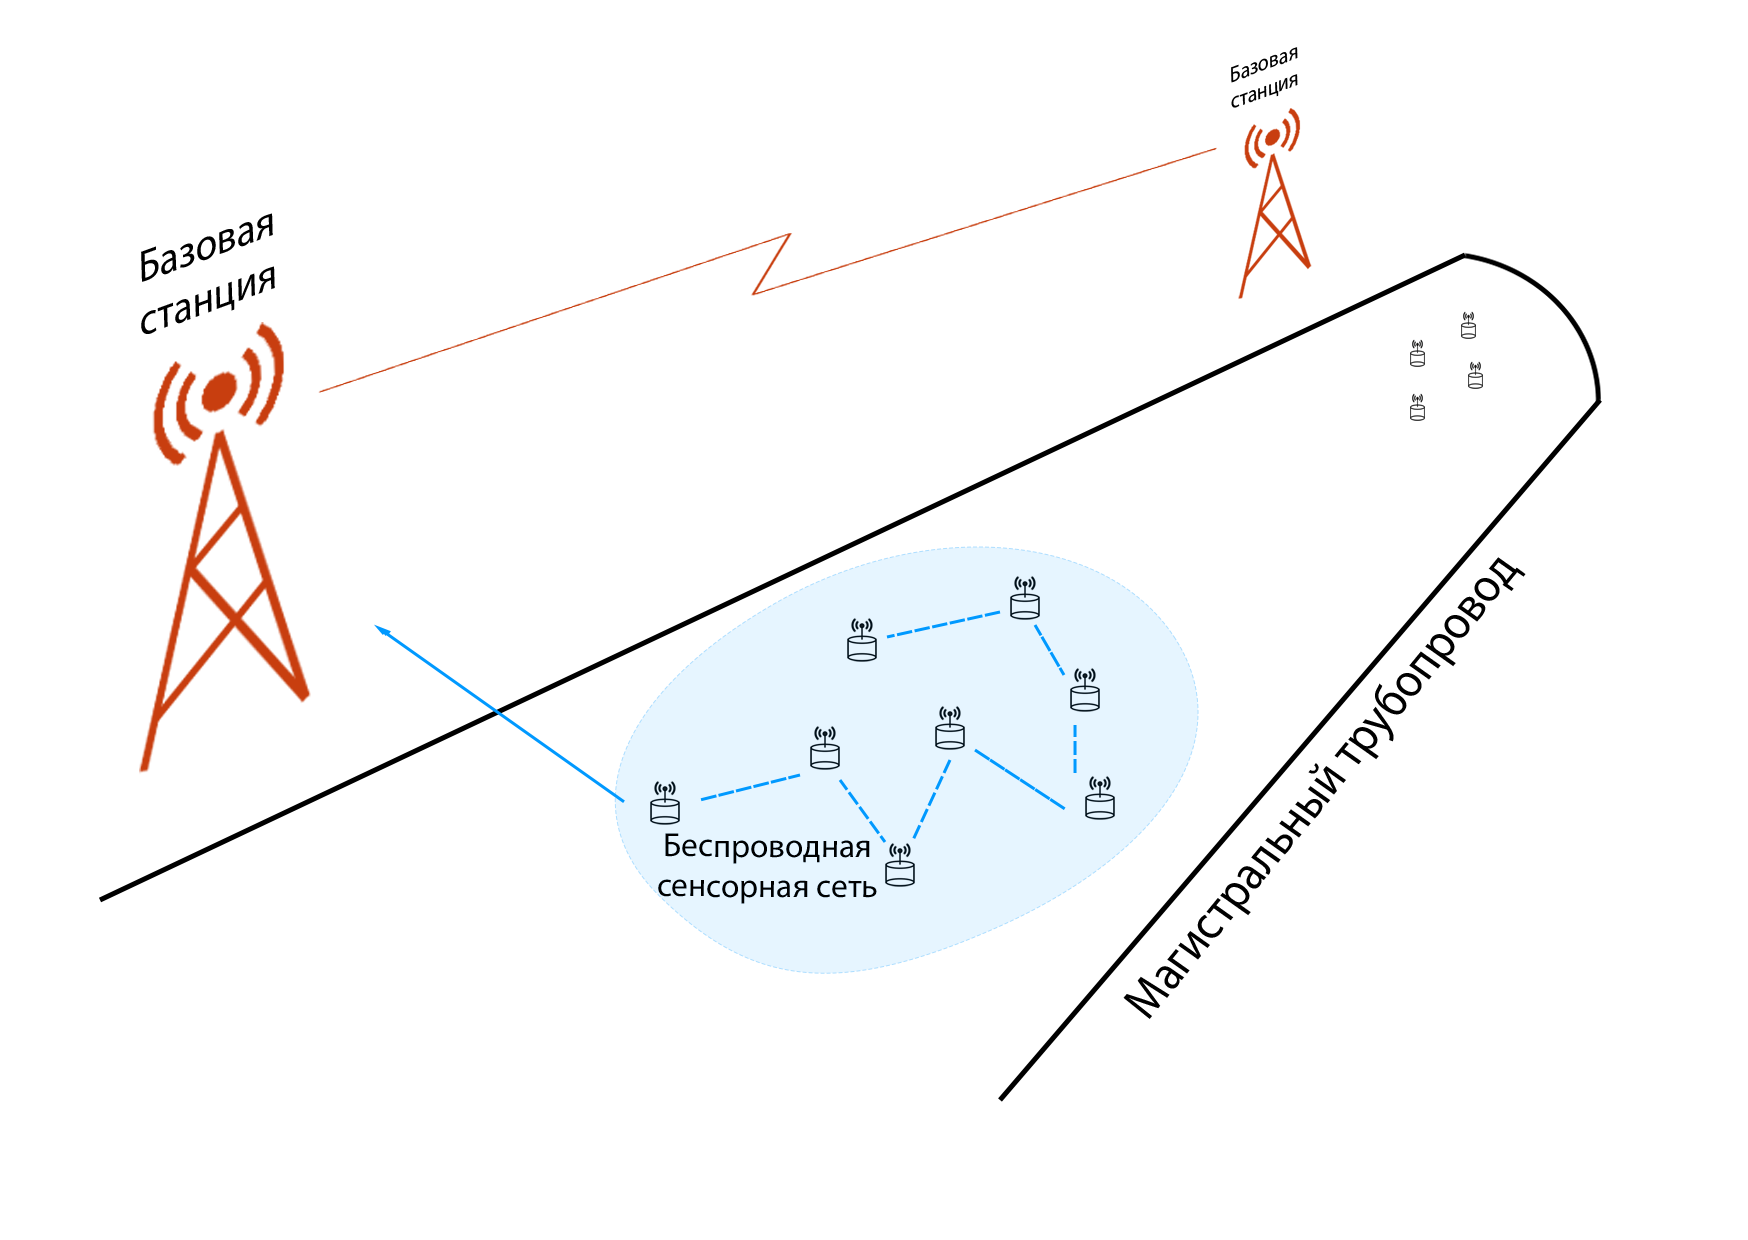
\includegraphics[scale=1.1]{pipeline.png}
  }
  \caption{Беспроводная сеть вдоль магистрального трубопровода}\label{fig:part2_pipeline}
\end{figure}

В \cite{Anupama2014, Jawhar2007} авторы предлагают иерархическую сенсорную сеть для мониторинга трубопроводов, в которой третий уровень иерархии сети представлен базовыми станциями, покрывающими весь линейный участок.

Один из современных методов обнаружение утечек и мониторинга в реальном времени является использование беспроводной сети связи на базе стационарных объектов -- базовых станций и  беспилотных летательных аппаратов  (БПЛА, Unmanned Aerial Vehicle, UAV) \cite{Aljuaid2020}. В \cite{Fedorova2020} рассматривается использование БПЛА для мониторинга нефтепроводов. Предлагается математическая модель для определения состава группы БПЛА и метода ее базирования.

Еще одним немаловажным линейным объектом любого промысла, требующим постоянного контроля является сеть промысловых дорог. С учетом большой удаленности друг от друга объектов нефтегазовой отрасли друг от друга целесообразно организовать телекоммуникационную сеть вдоль протяженных автодорог для контроля данного линейного участка с помощью информации с систем видеонаблюдения \cite{Vish2015} (Рисунок \ref{fig:part2_roadisdeunit}). Одним из наиболее перспективных решений на транспортных участках является организация автомобильных сетей (Vehicular ad hoc network, VANET) \cite{Massobrio2020, Campolo2015}. Для решения данной проблемы хорошо подходит БШС. Организации БШС вдоль автодорог посвящено ряд зарубежных и отечественных работ. 

\begin{figure}[ht]
  \centerfloat{
      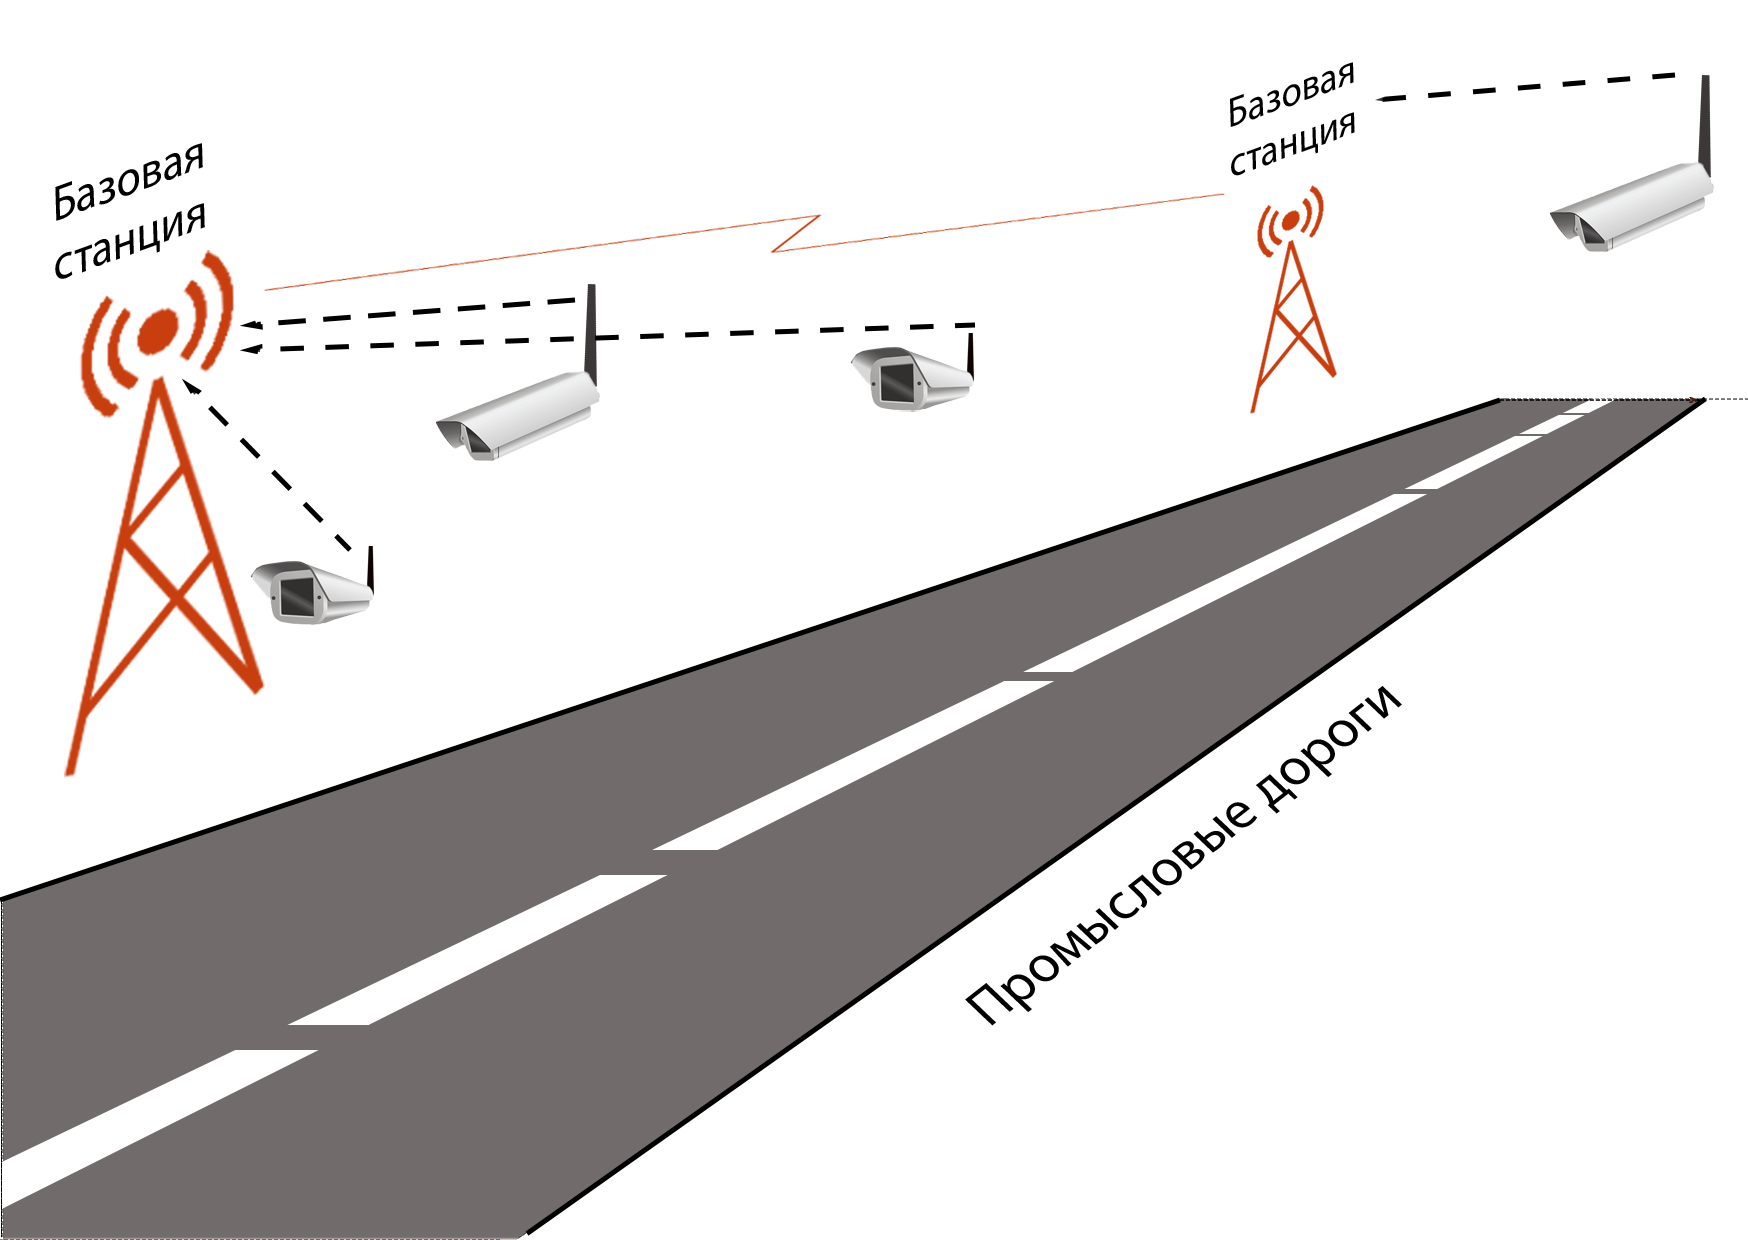
\includegraphics[scale=1.1]{roadsideunit.png}
  }
  \caption{Беспроводная сеть вдоль промысловых дорог}\label{fig:part2_roadisdeunit}
\end{figure}






Размещение БС вдоль линейного участка приобретают все большую актуальность на сегодняшний день. Большиство работ касаются проблемы размещения придорожных объектов (Roadside Unit, RSU) или другими словами БС вдоль автодорог. 

Задача оптимального размещения БС нашла свое широкое отражениие в исследованиях зарубежных и отечетсвенных авторов. Большиство работ касаются проблемы размещения придорожных объектов (Roadside Unit, RSU) или другими словами БС вдоль автодорог. В \cite{Cavalcante2012} предложена модель, используюящая генетический алгоритм для решения задачи о максимальном покрытии. Максимизация покрытия БШС с учетом ограничения стоимости БС представлена в работах \cite{BenBrahim2014, Vishnevsky2016_optimization}. В работах \cite{Liu2014, Gao2018, Jalooli2019} предложены новый модели размещения БС с учетом характеристик трафика на участках. В \cite{Reis2014} представлена задача размещения БС для протокола IEEE 802.11p/Wave. В \cite{Guerna2021} предложена модель размещения БС с помощью муравьиного алгоритма. В работах \cite{Cavalcante2012, Liu2017} в качестве ограничений учитываются временные ограничения при размещения БС. В \cite{Bao2018} предлагают жадный алгоритм для минимизации RSU c условием ограничения задержек между любыми двумя узлами сети. В работе \cite{Ivanov2018} представлена задача размещения RSU вдоль линейного участка протяженной автомагистрали. 


Представление задачи размещения БС вдоль автодорог в виде одномерной задачи нашло свое широкое применение \cite{Ivanov2018, Reis2014, Vishnevsky2016_optimization, Liu2014, Gao2018, Jalooli2019, Zhang2017}. В нашем случае является также эффективным для применения вдоль промысловых дорог между удалленными на большие расстояния объектами нефтегазовых отрасли.

Задача размещения также актуально для беспроводных сетей. В работе \cite{Alduraibi2016} предложены модели размещения узлов беспроводной сенсорной сети (WSN, Wirelss Sensor Network), максимизирующий покрытие линейного участка трубопровода. В \cite{Aria2020} авторы представляют во внимание модель размещения узлов WSN обнаружения повреждений на трубопроводе, учитывающие зоны, которые будет контролировать только обслуживания персонал. В работах \cite{Hussein2020, Varshney2018, Varshney2021} представлены модели размещения узлов WSN минимизирующее суммарное энергопотребление. В \cite{Li2020, Albaseer2019} предложен модели кластеризации узлов БШС, в \cite{Albaseer2019} предлагают модели БШС для мониторинга утечек вдоль нефте-- и газопроводов.

В отличие от большинства реализаций БШС вдоль трубопроводов, где используется одноуровневая реализация сети, в данной диссертации, согласно широко используемой классификации \cite{Jawhar2009, Varshney2015, Abbas2018, Wang2011, Jawhar2013}, будет предложено иерархическая БШС сеть c линейной топологии. Данные с полевых измерительных устройств собираются шлюзом. Именно с этих шлюзов вся информация будет собираться через систему размещенных БС. В случае проектирования БШС для видеонаблюдения, вся поток будет идти на БС непосредственно с антенн камер видеонаблюдения. Для обеспечения масштабируемости сети и быстрое развертывание новых устройств, \fixme{в том числе мобильные обходчики} ставится задача максимального покрытия всего участка.


\section{Математические модели синтеза топологии сети для охвата линейного участка в виде задачи целочисленного линейного программирования}

В середине прошлого века с появлением первых компьютеров свою широкую популярность приобрела область математики, задачей корой является поиск экстремальных решений на допустимых множествах. Это положило начало математическому программированию. Сегодня наиболее важным классом задач математического программирования является задачи ЦЛП. Эти задачи формулируются как задачи линейного программирования (ЛП) с дополнительным ограничением целочисленности переменных. Для задач ЛП существуют полиномиальный алгоритм решения - симплекс-метод, предложенный Д. Данцигом \cite{Dantzig1963}. Добавленное ограничение целочисленности портит свойство выпуклости и полиномиальности \fixme{[Ссылка]}. Основная проблема, возникающая при решении практических задач на конечных множествах --  «проклятие размерности» \cite{Pershin2013}. C увеличением размерности пространства количества данных возрастает экспоненциально.

\fixme{Дописать}

Класс задач ЦЛП обладают замечательным свойством, их решения всегда целые при целых правых частях системы условий \cite{Pershin2013}. Следовательно, задачи такого рода можно решать как задачи линейного программирования, сняв условие целочисленности переменных. 

Существуют готовые коммерческие продукты, которые быстро считают задачу, наиболее популярные из них можно выделить MatLab Optimization ToolBox, Gurobi Optimize, GLPK, CPLEX.

% В данной секции будет представлена математическая модель в виде задачи целочисленного линейного программирования. Решение 

\subsection{Постановка задачи}

Проблема формулируется следующим образом. Для контроля над заданным линейным участком необходимо разместить базовые приемопередающие станции таким образом, чтобы максимизировать покрытие с ограничением на суммарную стоимость размещенных станций. Необходимо, чтобы любая БС в сети могла быть связана со шлюзами на концах участка через систему размещенных станций.

Задано множество станций $S = \{s_j\}$. Каждой станции приписаны параметры $s_j = \{r_j, \{R_{jq}\}, c_j \}$, $j = \overline{1,m}; q = \overline{1,m}; q \neq j$. Здесь $r_j$ -- радиус покрытия станции, $R_{jq}$ -- это радиус связи между станцями $s_j$ и $s_q$, и $c_j$ -- это стоимость. 

Задан линейный участок длиной $L$ с концами в точка $a_0$ и $a_{n+1}$. Внутри  отрезка $[a_0, a_{n+1}]$ задано конечное множество точек $A=\{a_i\}, i=\overline{1,n}$; эти точки соответствуют набору свободных мест, где могут быть размещены станции. Каждая точка $a_i$ определяется своей одномерной координатой $l_i$.

Заданы станции специального вида $s_{m+1}$ -- шлюзы. Данные шлюзы размещены на концах $a_0$ и $a_{n+1}$ данного линейного участка . Для данных станций параметр радиуса покрытия $r_{m+1}=0$. Радиус связи и стоимость не заданы.

Требуется разместить станции таким образом, чтобы максимизировать покрытие с условием ограничения на суммарную стоимость $C$.


\subsection{Модель целочисленного линейного программирования}

Перед тем как перейти к постановке задачи оптимизации в виде модели целочисленного линейного программирования, необходимо подготовки параметры БС: радиус связи между станциями $R_{jq}$ и радиус телекоммуникационного покрытия $r_j$ с помощью уравнений расчета дальности связи, представленных в главе 1.



Пусть $y_i^+$ и $y_i^-$, $i= \overline{0,n+1}$ определяют охват покрытия (справа и слева, соответственно) станций, покрывающих точку $a_i$ (Рисунок \cref{fig:part3_station_coverage}). Параметры $y_i^+$ и $y_i^-$ могут принимать только неотрицательные целые значения.

Величины  покрытия для шлюзов $y_0^+, y_0^-, y_{n+1}^+, y_{n+1}^-$ равны 0.

\begin{figure}[ht]
  \centerfloat{
      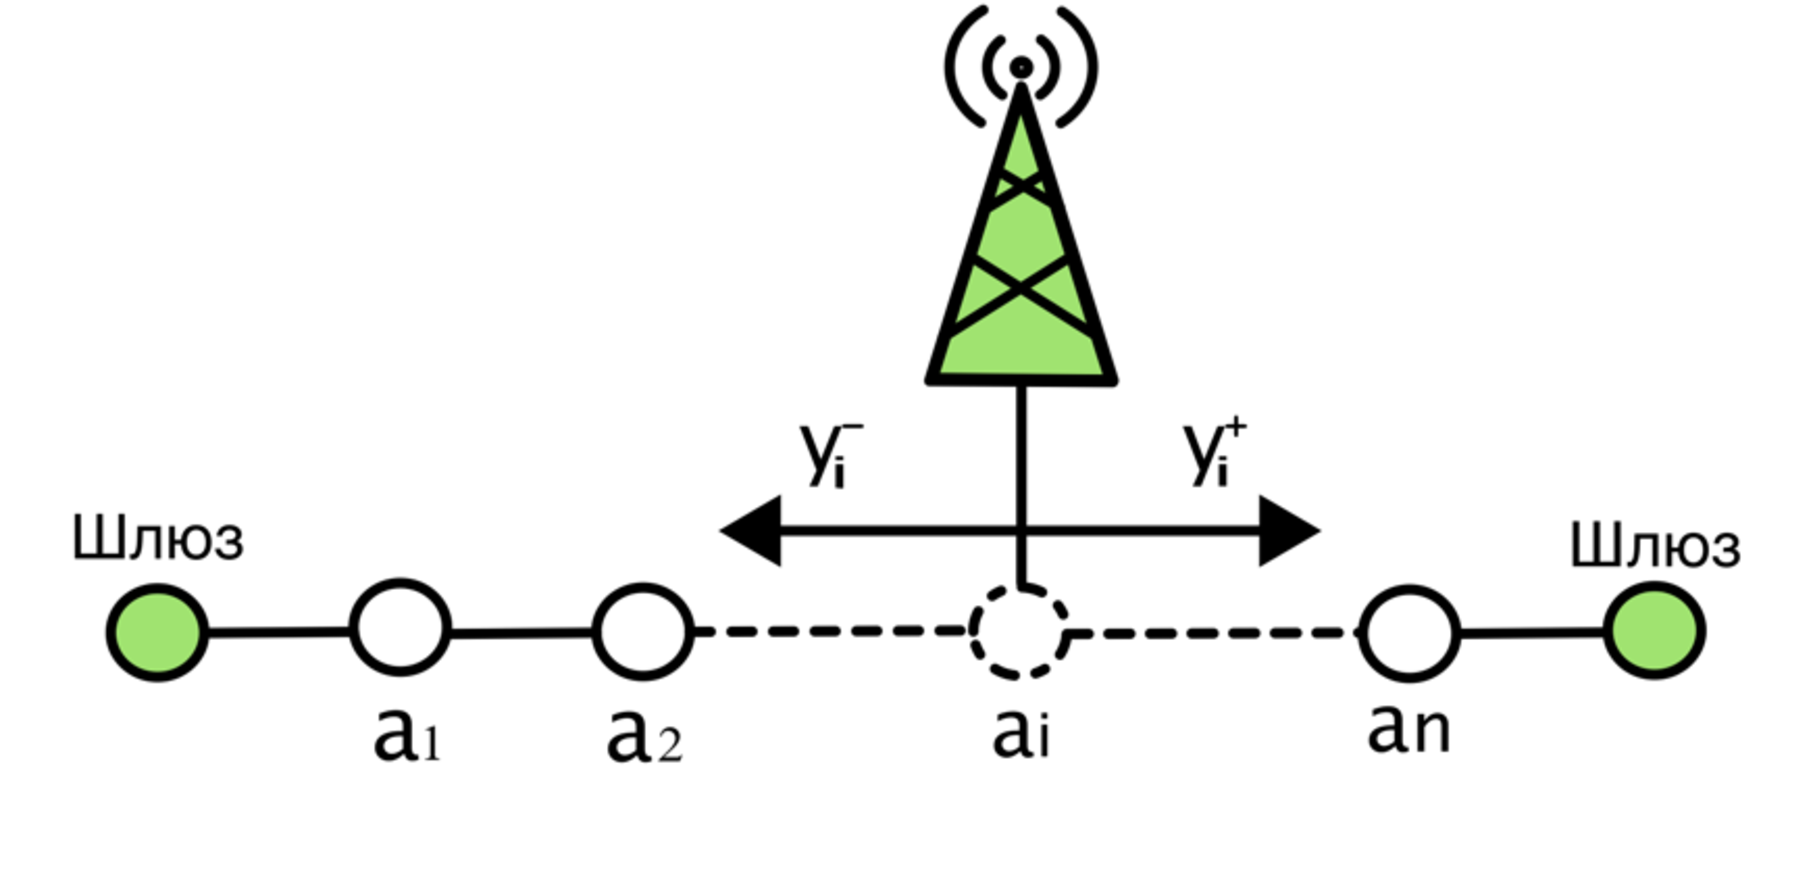
\includegraphics[scale=0.5]{station_coverage.pdf}
  }
  \caption{Охват покрытия станции}\label{fig:part3_station_coverage}
\end{figure}
 
Целевая функция будет представлена как:
\begin{equation}
  \label{eq:part3_objective_function}
  f =  \sum\limits_{i=1}^n (y_i^- + y_i^+) \rightarrow max
\end{equation}

Также введем бинарные переменные $x_{ij}$. Тогда $x_{ij}=1$, если станция $s_j$, размещенная на точке $a_i$, и $x_{ij}=0$ в противном случае; $i= \overline{1, n}$; $j = \overline{1,m}$.

Введем двоичные переменные $ e_i $. Тогда $ e_i = 1 $, если какая-либо станция находится в точке $ a_i $, и $ e_i = 0$  в противном случае; $ i = \overline {1, n} $. Для точек размещения шлюзов $ a_0 $ и $a_{n + 1}$ переменные $ e_0 = 1 $ и $ e_{n + 1} =1 $, соответственно. 

% Let us introduce binary variables $e_i$. Then $e_i$  is equal to 1, if any station is placed at point $a_i$ and $e_i$ is equal to 0 otherwise; $i = \overline{1, n}$. For gateways placement points $e_0$  is equal to 1 and $e_{n+1}$  is equal to 1.

Сформулируем следующую систему ограничений задачи.

По определению \cref{eq:part3_ei}:

\begin{equation}
  \label{eq:part3_ei}
  e_i =  \sum\limits_{j=1}^m x_{ij}, \quad i = \overline{1,n}. 
\end{equation}

Каждая станция должна быть размещена только в одной точке. \cref{eq:part3_xij}:

\begin{equation}
  \label{eq:part3_xij}
  \sum\limits_{i=1}^n x_{ij} \leq 1, \quad j = \overline{1,m}. 
\end{equation}

Значения покрытий не превышают радиус покрытия станции, размещенной в точке $ a_i $, и равны 0, если в точке $a_i$  нет станции \cref{eq:part3_yi_1, eq:part3_yi_2}:


\begin{equation}
  \label{eq:part3_yi_1}
  y_i^+ \leq \sum\limits_{j=1}^m x_{ij} \cdot r_j, \quad i = \overline{1,n};
\end{equation}

\begin{equation}
  \label{eq:part3_yi_2}
  y_i^- \leq \sum\limits_{j=1}^m x_{ij} \cdot r_j, \quad i = \overline{1,n}. 
\end{equation}

Общая область покрытия между любыми двумя точками $ a_i $ и $ a_k $, где расположены станции, не может превышать расстояние между этими точками \cref{eq:part3_yi_3, eq:part3_yi_4}.

\begin{equation}
  \label{eq:part3_yi_3}
  y_i^+ + y_k^- \leq \frac{l_k - l_i}{2} \cdot (e_i + e_k ) + (2 - e_i - e_k ) \cdot L, \quad i = \overline{1,n},  \quad k = \overline{i+1,n+1};
\end{equation}

\begin{equation}
  \label{eq:part3_yi_4}
  y_i^- + y_k^+  \leq \frac{l_i-l_k}{2} \cdot (e_i + e_k) + (2 - e_i - e_k) \cdot L, \quad i = \overline{1,n}, \quad k = \overline{i-1,0},
\end{equation}
где $ l_k $ и $ l_i $ - координаты точек $ a_i $ и $ a_k $, соответственно. Это условие исключает влияние пересечений покрытий станций при вычислении общего значения покрытия между станциями (Рисунок \cref{fig:part3_total_coverage_between_points}).

\begin{figure}[ht]
  \centerfloat{
      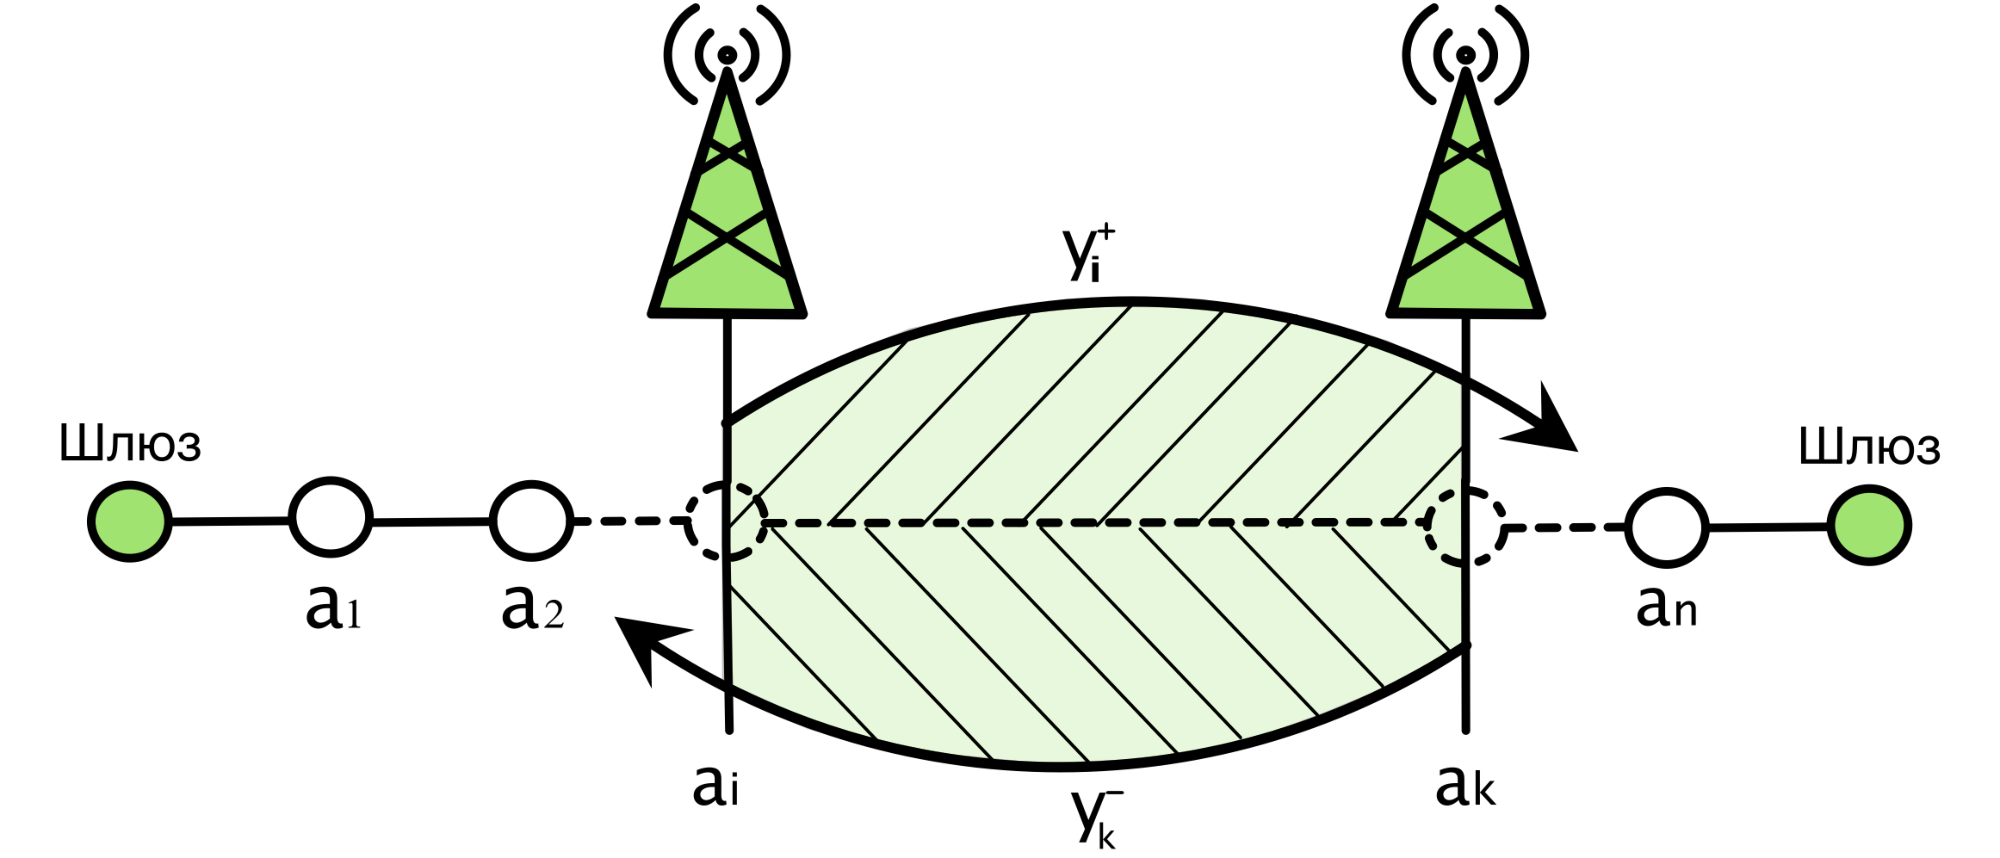
\includegraphics[scale=0.5]{total_coverage_between_points.pdf}
  }
  \caption{Область покрытия между любыми двумя точками}\label{fig:part3_total_coverage_between_points}
\end{figure}

Согласно условиям задачи, станция, расположенная в $ a_i $, должна быть связана хотя бы с одной станцией слева и одной станцией справа, включая станции на конечных точках $ a_0 $ и $a_{n + 1}$. 

Введем бинарные переменные $z_{ijkq}, i = \overline{1,n}; j= \overline{1,m}; k=\overline{1,n},  k \neq i; q= \overline{1,m}, q \neq j$.

Переменная $ z_ {ijkq} = 1$, если в точке $ a_i $ размещена станция $ s_j $ и данная станция связана со станцией $ s_q $, размещенная в точке $ a_k $; и $ z_ {ijkq} = 0 $ в противном случае.

Переменная $ z_{ij0(m + 1)} = 1$, если станция $ s_j $, размещенная в точке $ a_i $, связана со шлюзом $ s_{m + 1} $ в точке $ a_0 $; $ z_{ij0 (m + 1)} = 0 $ в противном случае.
 
Переменная $ z_{ij(n + 1)(m + 1)} = 1 $, если здесь находится станция $ s_j $ в точке $ a_i $ и она связана со шлюзом $ s_{m + 1} $ в точке $ a_{n + 1} $; $ z_{ij0(m + 1)} = 0 $  в противном случае.

Станции должны быть размещены в обеих точках $ a_i $ и $ a_k $, \cref{eq:part3_z_ijkq_1, eq:part3_z_ijkq_2}:

\begin{equation}
  \label{eq:part3_z_ijkq_1}
  z_{ijkq} \leq e_i , \quad i = \overline{1, n}; \quad j = \overline{1, m}; \quad k = \overline{1,n}, k \neq i; \quad q = \overline{1,m}, q \neq j;
\end{equation}


\begin{equation}
  \label{eq:part3_z_ijkq_2}
  z_{ijkq} \leq e_k , \quad k = \overline{1, n}; \quad j = \overline{1, m}; \quad i = \overline{1,n}, i \neq k; \quad q = \overline{1,m}, q \neq j.
\end{equation}

\fixme{ПЕРЕДЕЛАТЬ  УРАВНЕНИЯ ОГРАНИЧЕНИЯ УСЛОВИЯ СВЯЗИ МЕЖДУ СТАНЦИЯМИ}

% Необходимо, чтобы станция $ s_j $ в точке $ a_i $ была связана с  любой станцией, расположенной в точке $ a_k $, справа от $ a_i $ ($ k> i $) или с правым шлюзом $ s_{m + 1} $ \cref{eq:part3_z_ijkq_3_1, eq:part3_z_ijkq_3_2}. 

% \begin{equation}
%   \label{eq:part3_z_ijkq_3_1}
%   \sum\limits_{k=i+1}^{n} \sum\limits_{\substack{q = 1\\ q \neq j}}^m z_{ijkq} + z_{ij(n+1)(m+1)} = x_{ij} ,  \quad i = \overline{1, n}, \quad j = \overline{1, m}.
% \end{equation}


% Станция $ s_j $, размещенная в $ a_{n} $, справа связана толко со шлюзом $ s_{m + 1} $ на месте $ a_ {n+1}$ \cref{eq:part3_z_ijkq_3_2}. 

% \begin{equation}
%   \label{eq:part3_z_ijkq_3_2}
%   z_{nj(n+1)(m+1)} = x_{nj} \quad j = \overline{1, m}.
% \end{equation}

% Также станция должна быть связана с любой станцией, расположенной в точке $ a_k $ слева от точки $ a_i $ ($ k <i $) или с левым шлюзом $ s_{m + 1} $ \cref{eq:part3_z_ijkq_4_1, eq:part3_z_ijkq_4_2}.

% \begin{equation}
%   \label{eq:part3_z_ijkq_4_1}
%   z_{1j0(m+1)}= x_{ij}, \quad j = \overline{1, m};
% \end{equation}

% Станция $s_j$, размещенная в точке $a_{1}$ слева может быть связана только со шлюзом $s_{m+1}$, расположенном в точке $a_0$ \cref{eq:part3_z_ijkq_4_1}.

% \begin{equation}
%   \label{eq:part3_z_ijkq_4_2}
%   z_{ij0(m+1)} + \sum\limits_{k=1}^{i-1} \sum\limits_{\substack{q = 1\\ q \neq j}} z_{ijkq}= x_{ij}, \quad i = \overline{2, n}, \quad j = \overline{1, m}.
% \end{equation}

% Необходимо, чтобы станция $ s_q $ в точке $ a_k $ была связана с любой станцией справа, расположенной в точке $ a_i $ \cref{eq:part3_z_ijkq_5}.

% \begin{equation}
%   \label{eq:part3_z_ijkq_5}
%   \sum\limits_{i=k+1}^{n} \sum\limits_{\substack{j=1 \\ j \neq q}}^m z_{ijkq} = x_{kq} , \quad k = \overline{1, n-1}, \quad q = \overline{1, m};
% \end{equation}

% Кроме того, станция $ s_q $ в точке $ a_k $ подключена к любой станции слева, расположенной в точке $ a_i $ \cref{eq:part3_z_ijkq_6}. 

% \begin{equation}
%   \label{eq:part3_z_ijkq_6}
%   \sum\limits_{i=1}^{k} \sum\limits_{\substack{j=1 \\ j \neq q}}^m z_{ijkq} = x_{kq} , \quad k = \overline{2, n}, \quad q = \overline{1, m};
% \end{equation}

% Неравенства \cref{eq:part3_z_ijkq_1, eq:part3_z_ijkq_2} и равенства \cref{eq:part3_z_ijkq_3_1, eq:part3_z_ijkq_3_2, eq:part3_z_ijkq_4_1, eq:part3_z_ijkq_4_2, eq:part3_z_ijkq_5, eq:part3_z_ijkq_6} обеспечивают условие симметрии связи между базовыми станциями, расположенными в точках $ a_i $ и $ a_k $, $\forall i, k $ (Рисунок \cref{fig:part3_station_link}).
% \fixme{Скачать, что Zijkq это линк только в одну сторону и необходимо с обепечить связи с двух сторон.}

Стоит отметить, БШС работает в полудуплексном режиме. Переменная $z_{ijkq}$ говорит только о наличии связи для передачи от БС $s_j$ до БС $s_q$. Чтобы обеспечить связь в обоих направлениях, необходимо проверять условия для  $z_{ijkq}$ (от $s_j$ до $s_q$) и для $z_{kqij}$ (от $s_q$ до $s_j$).

Необходимо обеспечить коммуникационную связь справа от БС \cref{eq:part3_z_ijkq_1_1, eq:part3_z_ijkq_1_2}. Станция $ s_j $ в точке $ a_i $ должна быть связана с  любой станцией, расположенной в точке $ a_k $, справа от $ a_i $ ($ k> i $) или с правым шлюзом $ s_{m + 1} $ \cref{eq:part3_z_ijkq_1_1} 

\begin{equation}
  \label{eq:part3_z_ijkq_1_1}
  \sum\limits_{k=i+1}^{n} \sum\limits_{\substack{q = 1\\ q \neq j}}^m z_{ijkq} + z_{ij(n+1)(m+1)} = x_{ij} ,  \quad i = \overline{1, n}, \quad j = \overline{1, m}.
\end{equation}
Требуется чтобы станция, размещенная справа от $s_j$ или правый шлюз $ s_{m + 1} $  были связаны с размещаемой станцией $ s_j $ \cref{eq:part3_z_ijkq_1_2}

\begin{equation}
  \label{eq:part3_z_ijkq_1_2}
  \sum\limits_{k=i+1}^{n} \sum\limits_{\substack{q = 1\\ q \neq j}}^m z_{kqij} + z_{(n+1)(m+1)ij} = x_{ij} ,  \quad i = \overline{1, n}, \quad j = \overline{1, m}.
\end{equation}

Необходимо обеспечить коммуникационную связь слева от БС \cref{eq:part3_z_ijkq_2_1, eq:part3_z_ijkq_2_2}. Станция $ s_j $ в точке $ a_i $ должна быть связана с  любой станцией, расположенной в точке $ a_k $, слева от точки $ a_i $ ($ k <i $) или с левым шлюзом $ s_{0}$ \cref{eq:part3_z_ijkq_2_1} 

\begin{equation}
  \label{eq:part3_z_ijkq_2_1}
  z_{ij0(m+1)} + \sum\limits_{k=1}^{i-1} \sum\limits_{\substack{q = 1\\ q \neq j}}^m z_{ijkq}= x_{ij}, \quad i = \overline{1, n}, \quad j = \overline{1, m}.
\end{equation}
Требуется чтобы станция, размещенная слева от $s_j$ или левый шлюз $ s_{0} $  были связаны с размещаемой станцией $ s_j $ \cref{eq:part3_z_ijkq_2_2}

\begin{equation}
  \label{eq:part3_z_ijkq_2_2}
    z_{0(m+1)ij} +  \sum\limits_{k=1}^{i-1} \sum\limits_{\substack{q = 1 \\ q \neq j}}^m z_{kqij}= x_{ij},  \quad i = \overline{1, n}, \quad j = \overline{1, m}.
\end{equation}


Неравенства \cref{eq:part3_z_ijkq_1, eq:part3_z_ijkq_2} и равенства \cref{eq:part3_z_ijkq_1_1, eq:part3_z_ijkq_1_2, eq:part3_z_ijkq_2_1, eq:part3_z_ijkq_2_2} обеспечивают условие симметрии связи между базовыми станциями, расположенными в точках $ a_i $ и $ a_k $, $\forall i, k $ (Рисунок \cref{fig:part3_station_link}).

\begin{figure}[ht]
  \centerfloat{
      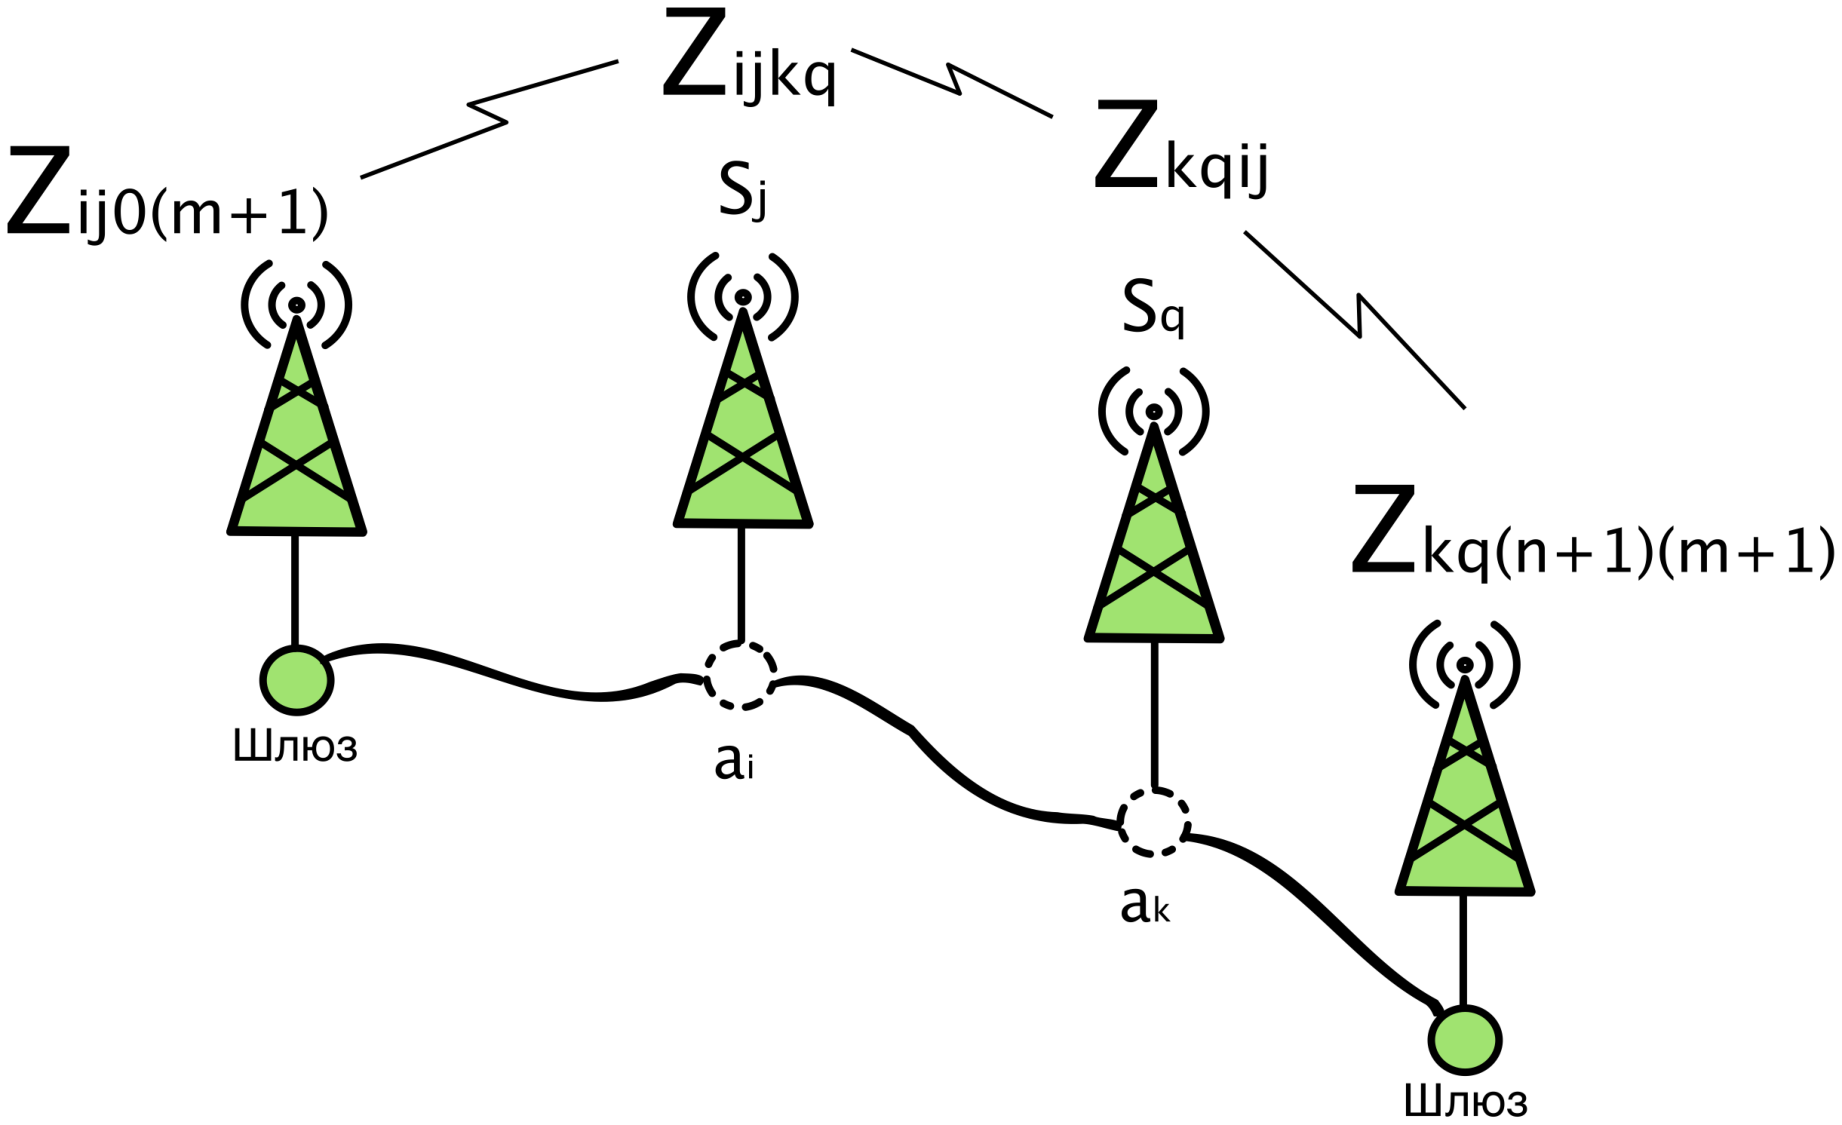
\includegraphics[scale=0.5]{station_link.pdf}
  }
  \caption{Связь между базовыми станциями}\label{fig:part3_station_link}
\end{figure}

Если станции $ s_j $ и $ s_q $ связаны, то максимальный радиус связи размещенных станций должен быть не меньше расстояния между точками $ a_i $ и $ a_k $, где расположены станции $ s_i $ и $ s_q $ (Рис. \cref{fig:part3_station_link_between_points}). Формально это можно записать как \cref{eq:part3_z_ijkq_3, eq:part3_z_ijkq_4}.

 $\forall i= \overline{1,n}$:
\begin{equation}
  \label{eq:part3_z_ijkq_3}
  z_{ijkq}(R_{jq}-(a_i-a_k ))\geq 0, \quad k=\overline{0,i-1}; \quad j=\overline{1,m}; \quad q= \overline{1,m}, q \neq j; 
\end{equation}

\begin{equation}
  \label{eq:part3_z_ijkq_4}
  z_{ijkq} (R_{jq}-(a_k-a_i )) \geq 0, \quad k=\overline{i+1,n+1}; \quad j=\overline{1,m}; \quad q= \overline{1,m}, q \neq j.
\end{equation}

\begin{figure}[ht]
  \centerfloat{
      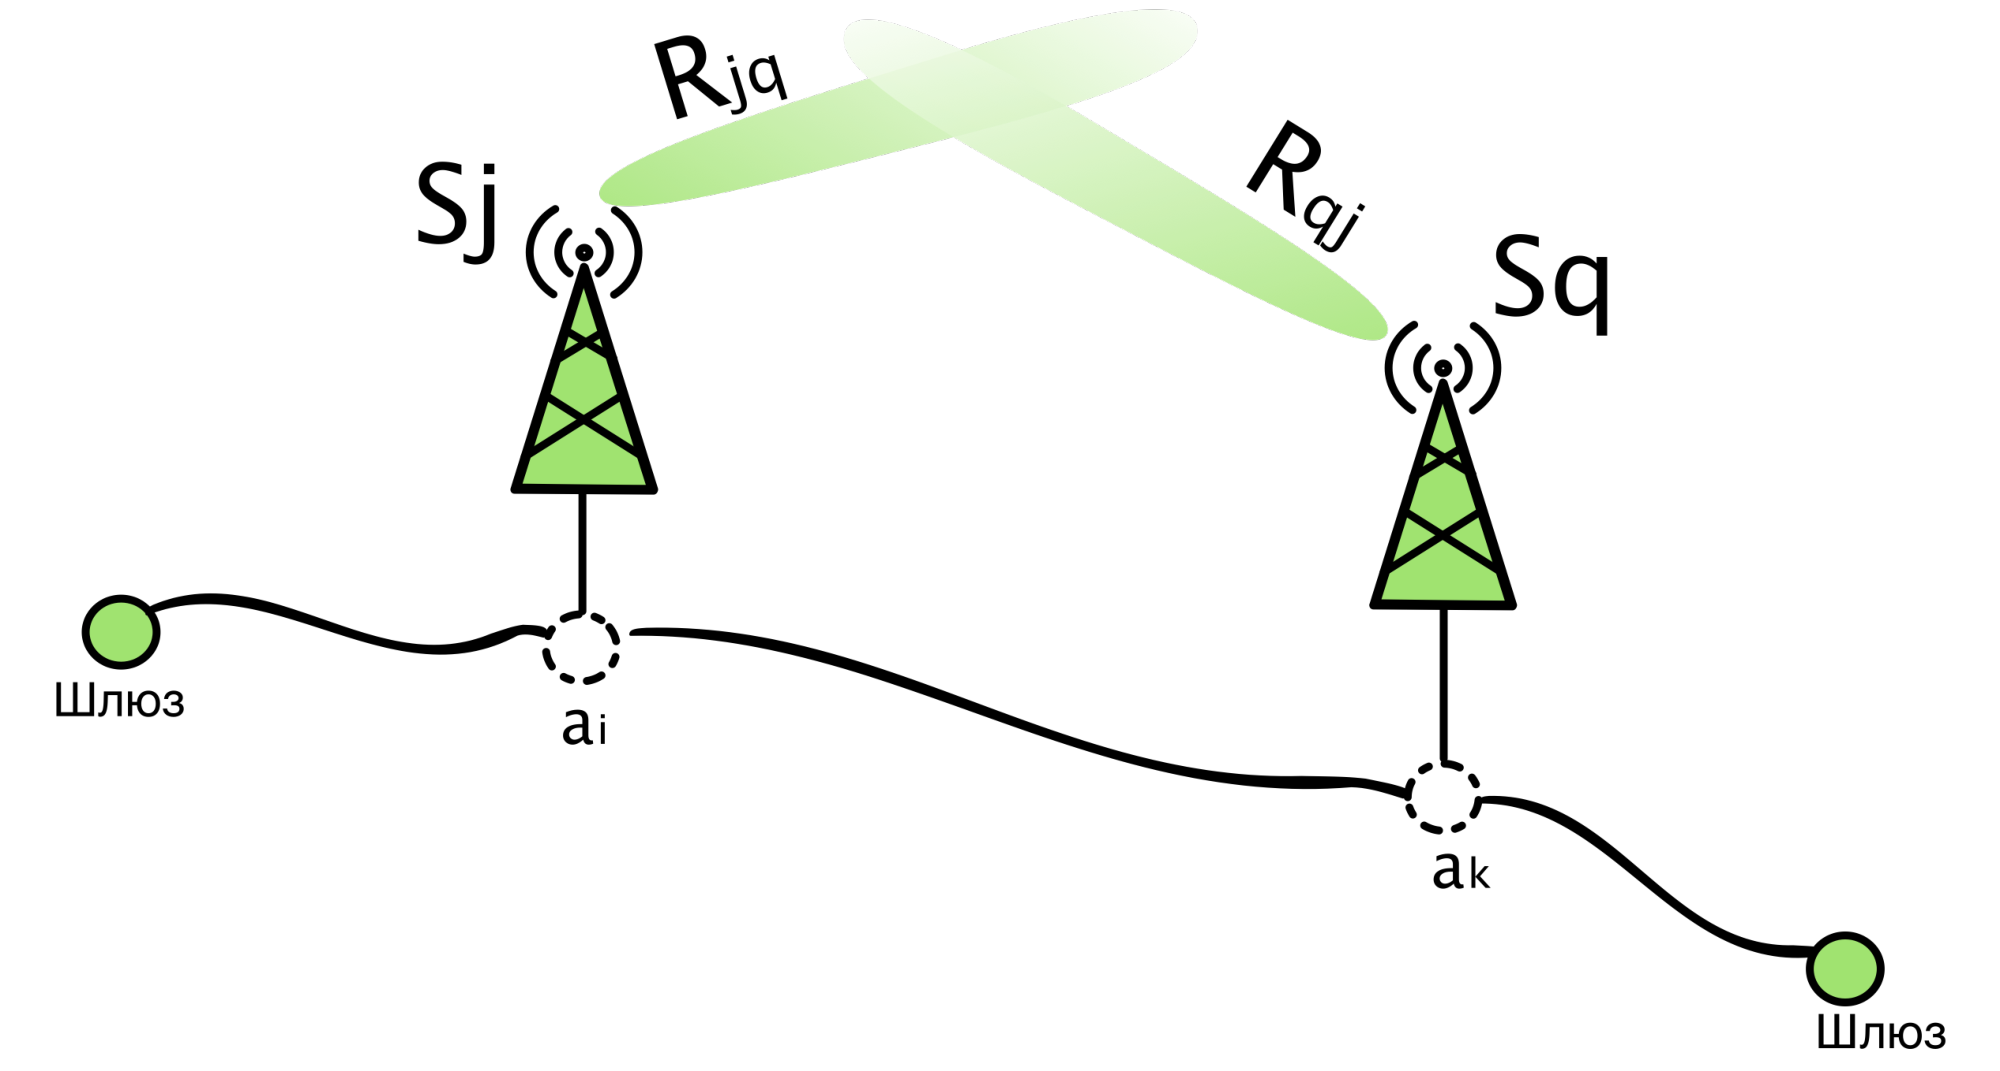
\includegraphics[scale=0.5]{station_link_between_points.pdf}
  }
  \caption{Обеспечение связи с соседней станцией}\label{fig:part3_station_link_between_points}
\end{figure}

Стоимость размещения должна удовлетворять бюджетному ограничению $C$:

\begin{equation}
  \label{eq:part3_cost}
  \sum\limits_{i=1}^n \sum\limits_{j=1}^m x_{ij} \cdot c_j \leq C.
\end{equation}

Работа \cite{Ivanov2018} содержит доказательство NP-трудности для частного случая задачи ЦЛП, когда вдоль линейной территории размещают множество однотипных станций с одинаковыми параметрами. Задача называется NP-трудной, если ей соответсвующая задача распознавания NP-полна \cite{Pershin2013}.  Представленная в данном исследовании модель \cref{eq:part3_objective_function} -- \cref{eq:part3_cost} рассматривает общий случай размещения, когда вдоль линейного участка размещают множество различных станций с разными техническими параметрами. Следовательно, данная задача является также NP-трудной.

Математическая модель рассчитывалась в пакете Optimization Toolbox MATLAB. Числовой пример решения полученной матемаческой модели задачи ЦЛП представлен в приложении \cref{app:ilp_solution}. В приложении также представлена методика расчета дальности связи для обеспечения коммуникации между базовыми станциями и охвата зоны покрытия.


\section{Математические модели синтеза топологии сети для охвата линейного участка в виде экстремальной задачи в комбинаторной форме}
\fixme{Пападимитриу X., Стайглиц К. Комбинаторная оптимизация: Алгоритмы и сложность}

\fixme{Эффективным способом повышения технико-экономических показателей при проектировании \fixme{БШС} является оптимизация топологии сети, а именно решение задачи выбора оптимального набора станций из заданного избыточного множества и определение мест их размещения вдоль линейной контролируемой территории.
Основным результатом работы, представленной в этой главе, является разработка итерационного метода выбора оптимальной топологии сети в процессе комплексного проектирования БШС. 
Принципиальной особенностью предлагаемого метода, повышающей его эффективность, является то, что для рассмотрения на этапе моделирования предлагается не одно решения, а последовательности лучших решений задачи оптимизации топологии сети. Это позволяет с помощью разработанной итерационной процедуры выбирать на этапе моделирования лучшее решение среди тех решений по топологии, которые удовлетворяют требуемым характеристикам проектируемой БШС.} 

\subsection{Постановка задачи}

Пусть задано множество станций $S=\{s_j\}$ с параметрами $s_j=\{r_j,\{R_{jq} \},p_j, c_j \},j=1,...,m;q=1,...,m;j \neq q $. Каждая БС содержит два модуля радиосвязи - для подключения абонентов и для связи с соседними станциями. Первая характеризуется параметром $r_j$ -- максимальный радиус покрытия станции, вторая характеризуется множеством $\{R_{jq} \}$ -- матрица радиусов связи между $j$-ой и $q$-ой базовыми станциями. Также заданы параметры: $p_j$ -- пропускная способность БС и $c_j$ -- стоимость станции.

Задана максимальная допустимая стоимость размещенных станций $C$. 


Задан отрезок $\alpha$ длины $L$ с концами в точках $a_0$ и $a_{n+1}$. Внутри отрезка $\alpha = [a_0, a_{n+1}]$ задано множество возможных точек размещения станций $A=\{a_i \},i=1,...,n$ с координатами $l_i$. Точка $a_0$ имеет координату $l_0=0$, точка $a_{n+1}$ имеет координату $l_{n+1}=L$. На концах отрезка в вершинах $a_0$ и $a_{n+1}$ стоят станции специального вида -- шлюзы $s_0$ и $s_{m+1}$, соответственно, для которых радиусы покрытия, пропускные способности и стоимости не задаются. Радиусы связи для обеспечения соединения с размещаемыми БС задаются как $R_{0j}$ и $R_{(m+1)j}$, соответственно.
Требуется разместить станции таким образом, чтобы максимизировать область покрытия отрезка $L$ при выполнении требования наличия связи каждой станции со станциями на концах отрезка (шлюзами) через систему размещенных станций, а также выполнении ограничений на величину межконцевой задержки $T$ и суммарную стоимость размещенных БС $C$.

Сформулируем задачу в виде экстремальной задачи на конечном множестве.

\textbf{Допустимой расстановкой станций} назовем такой возрастающий по величине координат $l_i$  набор пар $P = \{a_i, s_j\},a_i \in A,i \neq 0,i \neq n+1;s_j \in S$, для которого выполняются \textbf{требования}:

\begin{enumerate}
  \item  Для каждой пары $(a_i,s_j)$:
      \begin{enumerate}
          \item слева: либо найдется такая пара $(a_k,s_q)$, что, $l_i - l_k \leqslant R_{jq}$  и $l_i - l_k  \leqslant R_{qj}$, либо $l_i-l_0 \leqslant R_{j0}$ и $l_i - l_0 \leqslant R_{0j}$;
          \item справа: либо найдется такая пара $(a_t,s_g)$, что, $l_t-l_i \leqslant R_{jg}$ и $l_t - l_i \leqslant R_{gj}$, либо $l_{n+1}-l_i \leqslant R_{j(m+1)}$ и $l_{n+1}-l_i \leqslant R_{(m+1)j}$. 
\end{enumerate}
Данное требование гарантирует, что любая станция может быть связана со станциями на концах отрезка либо через промежуточные станции, либо непосредственно;
  \item Сумма задержек по всем размещенным станциям меньше заданной величины $T$ – средней межконцевой задержки по времени по всей системе станций:
  \begin{displaymath}
      \label{eq:part3_e2e_delay}
      \sum\limits_{j \in S_\sigma} \overline{T_j} \leqslant T,
  \end{displaymath}
где $S_\sigma$ – множество размещенных станций, $\overline{T_j}$ -- среднее время задержки на станции. Расчет задержек описан в параграфе \cref{part4_e2e_delay_section}
  \item Суммарная стоимость размещенных станций меньше заданного бюджетного ограничения  $C$.
\end{enumerate}

% \begin{enumerate}
%     \item  Для каждой пары $(a_i,s_j)$:
%         \begin{enumerate}
%             \item слева: либо найдется такая пара $(a_k,s_q)$, что, $l_i - l_k \leqslant R_{jq}$  и $l_i - l_k  \leqslant R_{qj}$, либо $l_i-l_0 \leqslant R_{j0}$ и $l_i - l_0 \leqslant R_{0j}$;
%             \item справа: либо найдется такая пара $(a_t,s_g)$, что, $l_t-l_i \leqslant R_{jg}$ и $l_t - l_i \leqslant R_{gj}$, либо $l_{n+1}-l_i \leqslant R_{j(m+1)}$ и $l_{n+1}-l_i \leqslant R_{(m+1)j}$. 
%   \end{enumerate}
% Данное требование гарантирует, что любая станция может быть связана со станциями на концах отрезка либо через промежуточные станции, либо непосредственно;
%     \item В одной точке стоит не более одной станции;
%     \item Сумма задержек по всем размещенным станциям меньше заданной величины $T$ – средней межконцевой задержки по времени по всей системе станций:
%     \begin{displaymath}
%         \label{eq:part3_e2e_delay}
%         \sum\limits_{j \in S_\sigma} \overline{T_j} \leqslant T,
%     \end{displaymath}
% где $S_\sigma$ – множество размещенных станций, $\overline{T_j}$ -- среднее время задержки на станции. Расчет задержек описан в параграфе \cref{part4_e2e_delay_section}
%     \item Суммарная стоимость размещенных станций меньше заданного бюджетного ограничения  $C$.
% \end{enumerate}

Каждой допустимой расстановке станций $P$ соответствует величина покрытия $z(P)$, определяемая как суммарная длина всех таких участков $\tau,\tau \subset \alpha$, что каждая точка этих 
участков попадает в зону покрытия, по крайней мере, одной станции, входящих в набор пар $P$.

Для удобства описании в дальнейшем алгоритмов введем понятие «недопокрытия» отрезка $\alpha$:

\begin{displaymath}
    f(P) = L - z(P)
\end{displaymath} 

Пусть $G$ -- множество всех допустимых расстановок $P$.
Тогда мы можем сформулировать нашу задачу в следующей комбинаторной форме экстремальной задачи на конечном множестве. 

\underline{\textit{\textbf{Задача 1.}}}

Требуется найти такую допустимую расстановку  $P^*$, что
\begin{equation}
    \label{eq:part3_P}
    P^* = \argmin \limits_{P \in G} f(P)
\end{equation}

Обозначим через $\Gamma$ все множество вариантов размещения станций (необязательно допустимых) из множества $S$ на заданном множестве возможных мест их размещения.

\subsection{Дерево ветвлений для перебора элементов в множестве \texorpdfstring{$\Gamma$}{Lg}}

Опишем процедуру построения бинарного дерева поиска (дерева ветвлений) для полного перебора без повторений всех элементов множества $\Gamma$. Данная процедура будет использована при построении дерева поиска в алгоритме МВиГ решения \textbf{задачи 1} \cite{SigalBook}.

Будем предполагать, что в множестве $S$ станции упорядочены по не убыванию радиусов покрытия.


Описываемая процедура использует известный прием разбиения множества $G$ на подмножества с использованием некоторого параметра. Процесс формирования и последовательность исследования подмножеств обычно представляется с помощью дерева поиска, представляющего собой ориентированное от корня «дерева ветвлений», где каждому подмножеству соответствует вершина на дереве. Множеству $\Gamma$ соответствует корневая вершина. 

\paragraph{Параметр для разбиения множеств на подмножества}

Выбор способа ветвления дерева связан со спецификой задачи. В случае \textbf{задачи 1} спецификой является размещение множества станций $S$ на множестве возможных точках размещения $A$. На каждом узле дерева будем применять дихотомическое ветвление.

\textit{\textbf{Процедура 1.}} Пусть $G_0$, где нижний индекс – номер итерации, исходное множество $\Gamma$. На каждой итерации, начиная с итерации $\nu=0$, разбиваем текущее подмножество $G_\nu$ на два подмножества $G^1_\nu$ и $G^2_\nu$. Множество $G_\nu$ обычно называется «материнским», а множества $G^1_\nu$  и $G^2_\nu$  - «потомками» множества $G_\nu$ или дочерними узлами (Рисунок \cref{fig:part2_bst_child_nodes}.)

\begin{figure}[ht]
  \centerfloat{
      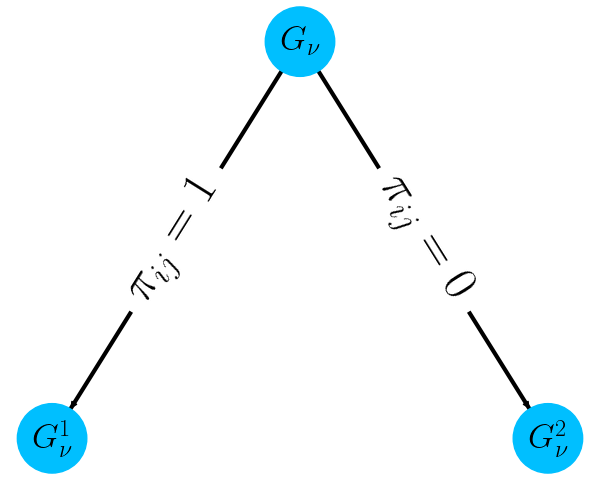
\includegraphics[scale=0.5]{bst_child_nodes.png}
  }
  \caption{Ветвление бинарного дерева}\label{fig:part2_bst_child_nodes}
\end{figure}

В качестве параметра разбиения используем переменную $\pi_{ij}$, принимающей два значения 0 и 1:

\begin{itemize}
    \item $\pi_{ij}=1$, если наложено условие, что на месте $a_i$ расположена станция $s_j$;
    \item $\pi_{ij} = 0$, если наложено условие, что на месте $a_i$ станция $s_j$  располагаться не будет.
\end{itemize}

В дальнейшем будем считать, что для множества $G^1_\nu$ задано условие $\pi_{ij}=1$, а для множества $G^2_\nu$  задано условие $\pi_{ij} = 0$.

Все дочерние множества удовлетворяют следующим условиям:

\begin{equation}
    \label{eq:part4_G_cup}
    G^1_\nu \cup G^2_\nu = G_\nu;
\end{equation}


\begin{equation}
    \label{eq:part4_G_cap}
    G^1_\nu \cap G^2_\nu = \varnothing.
\end{equation}

\textit{\textbf{Выбор переменной для разбиения на $\nu$-ой итерации}}

На этапе разбиения любого множества $G_\nu$ все множество переменных $\Pi = \{\pi_{ij}\}$ можно разделить на три подмножества: 

\begin{itemize}
  \item $\Pi^+$ -- «фиксированные» переменные, для которых $\pi_{ij}=1$;
  \item $\Pi^-$ -- «запрещенные» переменные, для которых $\pi_{ij}=0$;
  \item $\Pi^f$ -- «свободные» переменные, для которых значения на данной итерации еще не заданы.
\end{itemize}
Правило выбора переменной для разбиения множества $G_\nu$. Для разбиения множества $G_\nu$ на каждой итерации выбирается переменная из множества $\Pi^f$ c наименьшим индексом $j$ среди всех переменных с наименьшим индексом $i$. Таким образом, сначала определяется незанятое место размещения $a_i$ с наименьшим номером (индексом $i$) и на нем размещается еще не размещенная станция $s_j$ с наименьшим номером (индексом $j$).

\paragraph{Движение по дереву ветвлений.}

После разбиения очередного подмножества $G_\nu$ на два подмножества $G^1_\nu$  и $G^2_\nu$, последним на дереве ветвлений присваиваются порядковые индексы $G_{\nu+1}$ и $G_{\nu+2}$, соответственно (Рисунок \ref{fig:part2_tree_traversal}).
При формировании дерева ветвлений различаются два типа шагов: «прямой» и «обратный». Прямой шаг -- это движение «в глубину» по той же ветви дерева, реализующее очередное разбиение множества $G_\nu$ на два потомка, и обратный шаг, реализующий переход от множества $G_\nu$  к одному из ранее сформированных подмножеств. Обратный шаг делается в том случае, когда: либо получено множество $G_\nu$, состоящее из единственного элемента, либо множество $G_\nu$  при данном наборе значений переменных $\pi_{ij}$, выделяющих данное подмножество $G_\nu$ из множества $G_0$, пусто. В этих случаях соответствующая вершина дерева называется «закрытой».

\begin{figure}[ht]
  \centerfloat{
      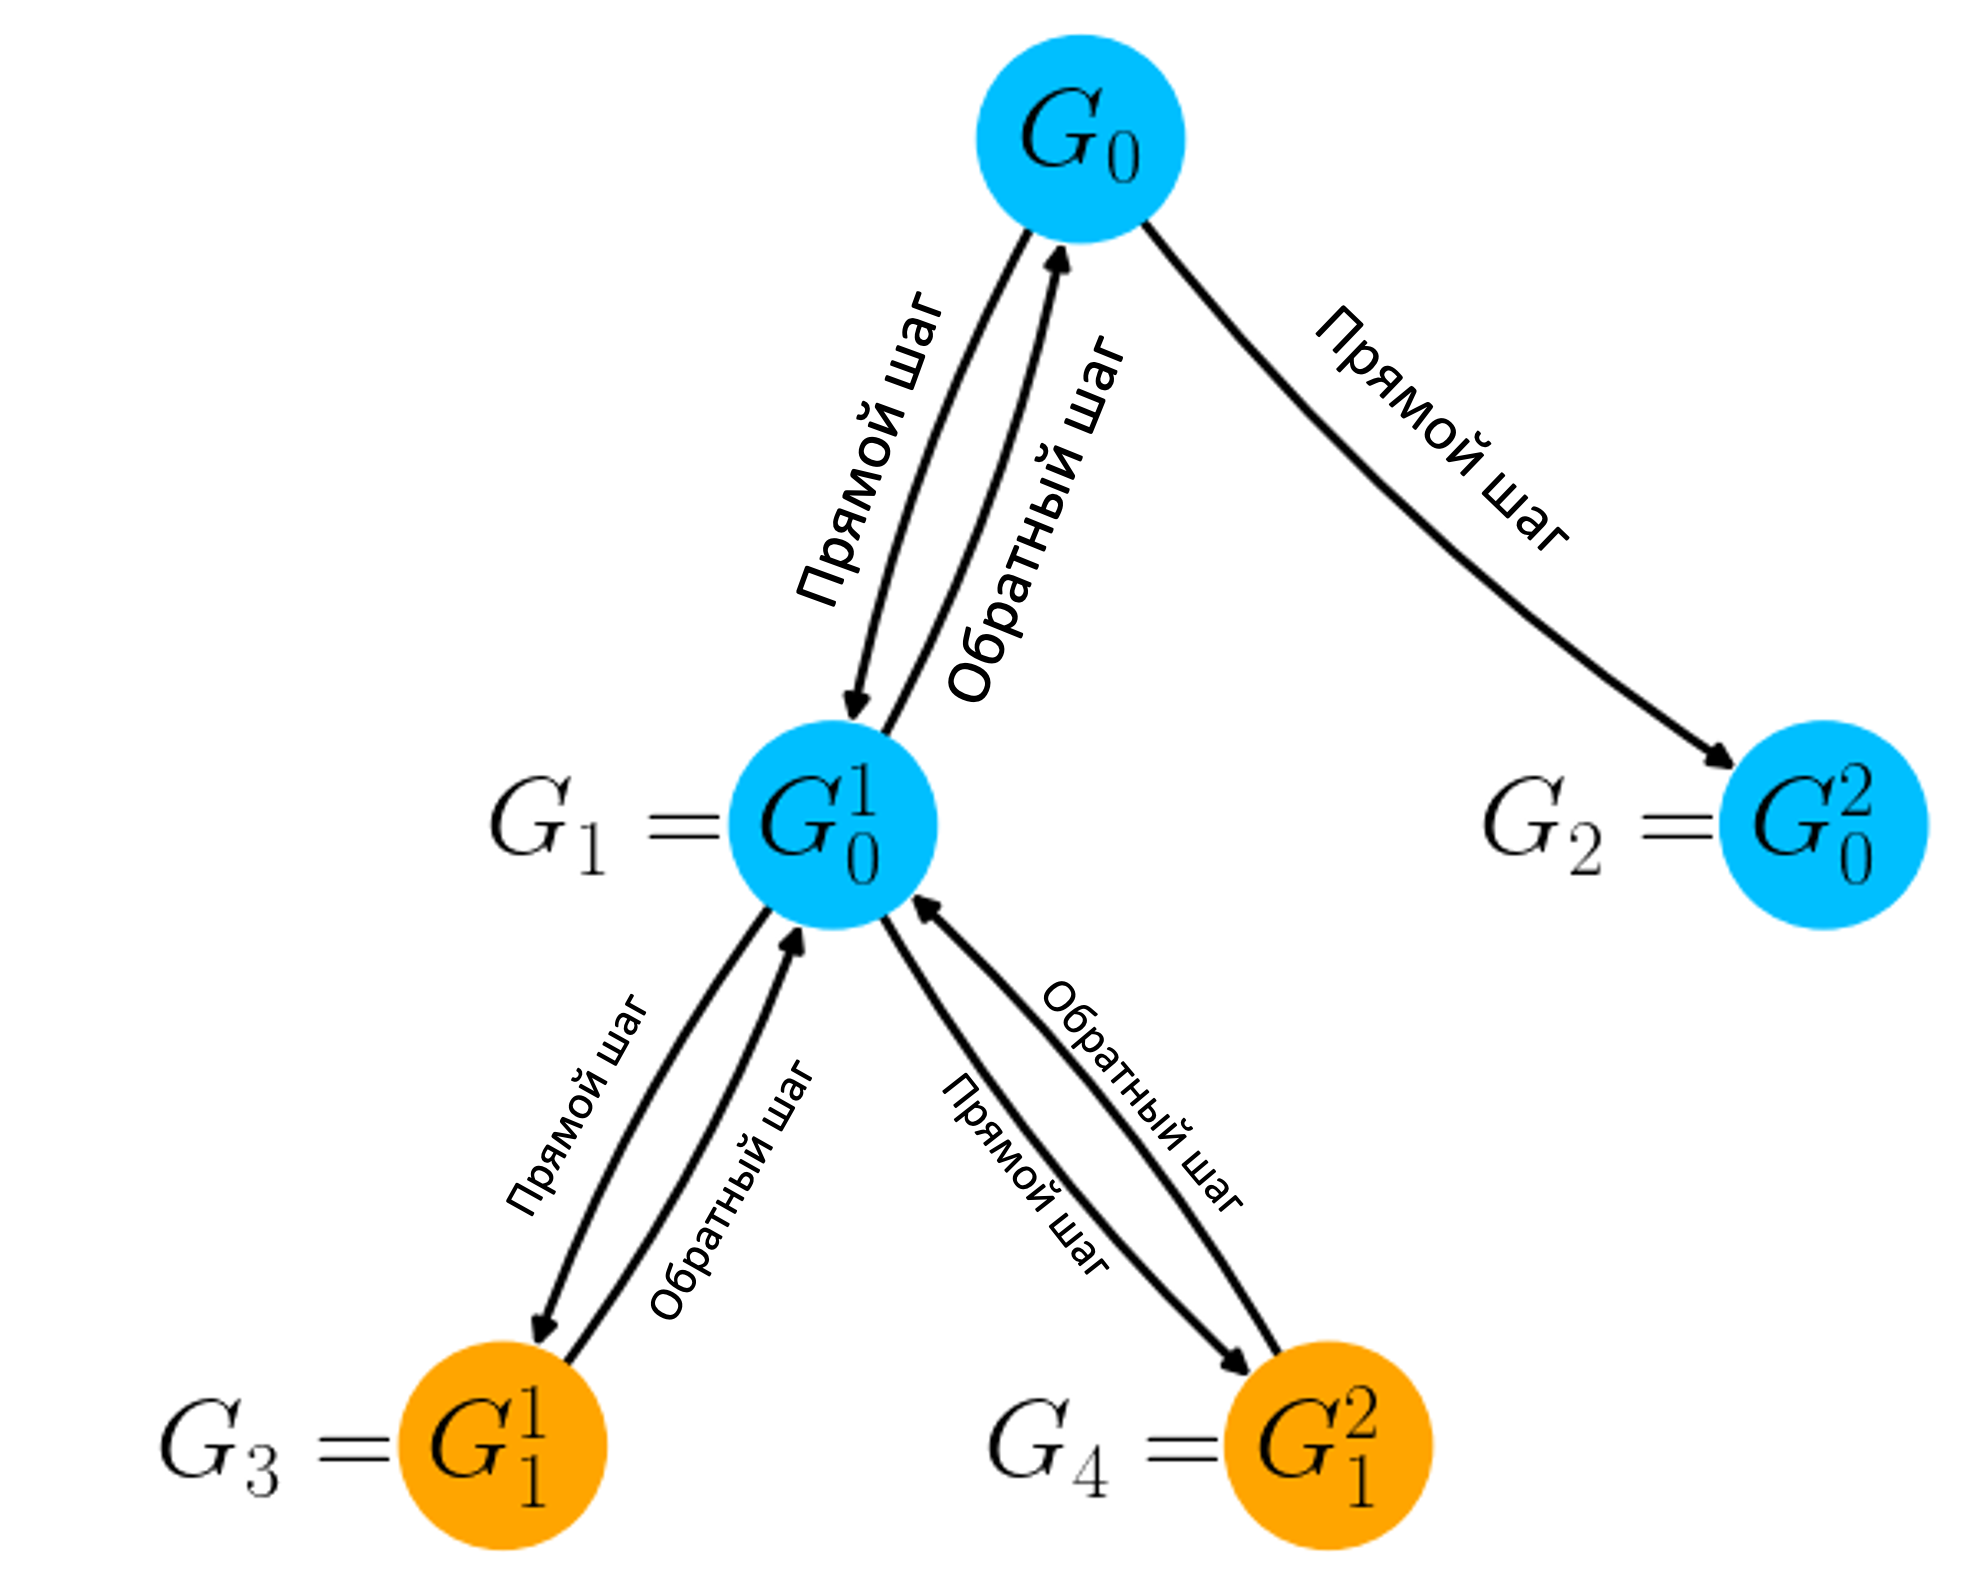
\includegraphics[scale=0.8]{tree_traversal.png}
  }
  \caption{Движение по дереву поиска}\label{fig:part2_tree_traversal}
\end{figure}

Для движения по дереву будем использовать правило \fixme{LIFO}. На основании этого правила прямые шаги будут выполняться до тех пор, пока не будет получена закрытая вершина. На дереве ветвлений это соответствует продолжению движения по той же ветви дерева. При этом из двух множеств $G^1_\nu$  и $G^2_\nu$ первым будет исследоваться на возможность закрытия соответствующей вершины множество $G^1_\nu$. Если вершина не будет закрыта, то из неё будет продолжено дальнейшее движение по той же ветви (выполнение прямого шага). Если вершина будет закрыта, то будет выполнен обратный шаг: для продолжения движения будет выбрана незакрытая вершина с наибольшим порядковым номером $\nu$ среди всех висячих вершин дерева (последняя сформированная вершина из нерассмотренных). Процедура будет завершена, когда все вершины дерева будут закрыты.

Заметим, что выполнение условий \cref{eq:part4_G_cup, eq:part4_G_cap} гарантирует, что в результате завершения работы \textit{\textbf{процедуры 1}} будут просмотрены все элементы множества $\Gamma$ без повторений. Эти же условия определяют фундаментальное свойство дерева ветвлений: на каждой итерации объединение множеств $G_\nu$ всех висячих вершин дерева дает исходное множество $G_0$ корневой вершины.

\subsection{Метод ветвей и границ для задачи размещения БС} \label{BnB}
Для построения алгоритма \fixme{МВиГ} для решения \textbf{задачи 1} с использованием \textit{\textbf{процедуры 1}} для построения дерева ветвлений достаточно разработать методы исследования вершин дерева на возможность их закрытия.

В соответствии с техникой \fixme{МВиГ} закрытие вершины в результате исследования, соответствующего ей множества $G_\nu$ возможно в трех случаях.

\underline{\textit{\textbf{Случай 1.}}} Множество $G_\nu$ -- пусто, т.е. доказано, что в множестве $G_\nu$ при данном наборе фиксированных и запрещенных переменных $\pi_{ij}$ нет ни одной допустимой расстановки $P$.

\underline{\textit{\textbf{Случай 2.}}} Доказано, что в множестве $G_\nu$ не может быть допустимой расстановки P с меньшим значением целевой функции \cref{eq:part3_P}, чем у лучшей расстановки $\widehat{P}$ из уже найденных. Значение функции $f(\widehat{P})$ называется «рекордом», а расстановка $\widehat{P}$ -- «рекордным решением». В качестве начального рекорда принимается число заведомо большее искомого оптимального решения, например,  длина всего отрезка $L$.

\underline{\textit{\textbf{Случай 3.}}} Найдено оптимальное решение \textbf{задачи 1} на множестве $G_\nu$.
Прежде, чем рассмотреть эти три случая, запишем важное свойство любого множества $G_\nu$, являющееся следствием принятого правила выбора свободной переменной для разбиения очередного множества $G_\nu$ при прямом шаге. 

\textit{\textbf{Свойство 1.}} Пусть для исследуемого множества $G_\nu, \nu > 0$, точка $a_k$ -- любое из мест, на которых уже размещена станция из множества $S$ в соответствии с набором фиксированных и запрещенных переменных $\pi_{ij}$, выделяющим данное множество из множества $G_0$. Тогда для всех мест «слева» от $a_k$, т.е. точек $a_i$, $i<k$, размещение станций уже определенно (при этом некоторые места могут быть пустыми).
Перейдем непосредственно к исследованию \underline{\textit{\textbf{случаев 1 – 3}}}.

\underline{\textit{\textbf{Случай 1.}}}

Проверка текущего множества $G_\nu$ на пустоту состоит в установлении факта невозможности выполнения требования \fixme{1--3}, введенных ранее при определении допустимой расстановки.

% \fixme{Чтобы доказать  невыполнение требования 2 надо показать, что при данном наборе запрещенных и фиксированных переменных $\pi_{ij}$  для некоторой из еще не размещенной станции не существует свободного места размещения. Подобная проверка алгоритмически легко реализуема: достаточно показать, что существует такое $k$, что для станции $s_k$, не существуюет ни одной переменной $p_{ij}$ из множества $P^f$, другими словами не существует ни одного $a_i$, для которого $\pi_{ik} \neq 1$ и $\pi_{ik} \neq 0$.} 



\paragraph{Проверка выполнения условия связи между размещенными БС}

Построим алгоритм проверки выполнения требования 1.
% \fixme{Рассмотрим сначала исходное множество  $G_0 = \Gamma$. Необходимое условие выполнения требования 1: расстояния от точки $a_0$ до точки $a_1$ и от точки $a_n$  до точки $a_{n+1}$ должны быть не больше максимального радиуса связи между станциtq из множества $S$ и шлюзом, и расстояние между двумя любыми смежными точками $a_i, i=1,...n$, должно быть не больше чем радиус связи из оставшихся БС в множества $S$. сли в результате проверки оказывается, что эти условия не выполняются, то множество $G_0$ допустимых расстановок пусто и \textbf{Задача 1} не имеет решения.}


% Необходимое условие выполнения требования 1: расстояние между двумя любыми смежными точками $a_i, i=1,...n$, должно быть не больше, чем второй по величине после максимального радиус связи у заданного множества, а расстояния от точки $a_0$ до точки $a_1$ и от точки $a_n$  до точки $a_{n+1}$ должны быть не больше максимального радиуса связи среди радиусов связей станций множества $S$. Если в результате проверки оказывается, что эти условия не выполняются, то множество $G_0$ допустимых расстановок пусто и \textbf{Задача 1} не имеет решения.

Рассмотрим проверку условия выполнения требования 1 для  множества  $G_\nu, \nu>0$. 
Пусть множество $G_\nu$  образовано разбиением материнского множества при помощи переменной $\pi_{kt}=1$, и множество содержит более одного распределения $P$.
Алгоритм проверки состоит из \textbf{3 шагов}.

\textbf{Шаг 1}. Проверяем, что каждый из радиусов $R_{th}$ и $R_{ht}$, где $h$ – индекс станции, размещенной на ближайшей к точке $a_k$ слева точке $a_d$, больше расстояния $l_k-l_d$. 

\textbf{Шаг 2}. Проверяем, что как радиус $R_{tj}$, так и максимальный радиус $R_{jt}$ среди еще нераспределенных станций не меньше расстояния между точкой $a_k$ и ближайшей к ней точкой справа $a_i$.  Если все станции распределены, то множество $G_\nu$ состоит из единственного варианта распределения и этот случай будет рассмотрен далее.

\textbf{Шаг 3}. Проверяем, что, если количество нераспределенных станций больше 1, то расстояние между двумя любыми смежными точками $a_i, i=k+1,...,n$, не больше, чем второй по величине после максимального радиус связи у еще не распределенного множества станций, а расстояние между точками $a_{n+1}$ и $a_n$  не больше, чем максимальный радиус связи среди нераспределенных станций. Если осталась только одна нераспределенная станция, то проверяем, что среди еще незанятых точек справа от точки $a_k$  есть, по–крайней мере, одна такая точка, что расстояния от этой точки до точки $a_k$ и одновременно от этой точки до точки $a_{n+1}$ не больше, чем  радиус связи у нераспределенной станции.

Если в результате проверки оказывается, что, хотя бы на одном из шагов получен отрицательный результат, то множество $G_\nu$ -- пусто, соответствующая этому множеству на дереве поиска вершина должна быть закрыта и далее выполняется шаг обратного хода в соответствии с \textbf{Процедурой 1}.

Если множество $G_\nu$ образованно разбиением материнского множества при помощи переменной $\pi_{kt}=0$ и $a_v$ -- точка с наибольшим индексом, среди точек, на которых уже размещены станции (с учетом точки $a_0$ ), то надо проверить, что расстояние между точками $a_v$ и $a_k$ не больше, чем максимальный радиус среди радиусов связи у еще нераспределенных станций. Если проверка отрицательна, то множество $G_\nu$  - пусто, соответствующая этому множеству на дереве поиска вершина должна быть закрыта и выполняется шаг обратного хода в соответствии с \textbf{Процедурой 1}.

\fixme{Проверка требований 2 и 3 сводится к установлению факта непревышения суммарных величин стоимости и межконцевой задержки заданным ограничениям.}

\underline{\textit{\textbf{Случай 2.}}}
Построим оценку величины «недопокрытия» для множества $G_\nu$, полученного из материнского множества добавлением условия $\pi_{kt}=1$. Частичным «недопокрытием» назовем величину $\Delta(k,d,p,t)$, которая вычисляется по формуле:

\begin{equation}\label{eq:part4_delta}
\Delta(k,d,p,t) = max\{\left(a_{k} - a_{d} \right) - \left(r_{p} + r_{t} \right), 0\}.
\end{equation}

Частичное «недопокрытие» \cref{eq:part4_delta} определяется для любых двух точек $a_d$ и $a_k$ ($k>d$), на которых расположены станции $s_p$ и $s_t$ при условии, что между этими точками нет других станций. Для любой расстановки $P$ «недопокрытие» $f(P)$ вычисляется как сумма всех «недопокрытий» $\Delta(k,d,p,t)$ между местами размещения станций, включая концы отрезка $\alpha$, на которых стоят станции особого типа $s_0$ и $s_{m+1}$.

Построим нижнюю оценку $W(G_{\nu} )$ для недопокрытий $f(P)$ расстановок $P$ множества $G_\nu$, т.е. 

\begin{displaymath}
W(G_\nu) \leq f(P), P \in G_\nu. 
\end{displaymath}

Если $W(G_\nu) \geq f(\widehat{P})$, то множество $G_\nu$ не может содержать расстановки, лучше уже найденной расстановки $\widehat{P}$, тогда соответствующая множеству $G_\nu$  вершина на дереве поиска должна быть закрыта и далее выполняется шаг обратного хода в соответствии с  \textit{\textbf{процедурой 1}}. 

Построим оценку «недопокрытия» для множества $G_\nu$, полученного из материнского множества добавлением условия $\pi_{kt}=1$. Оценку будем искать в виде суммы

\begin{equation}
  \label{eq:part4_noncoverage_estimation}
  W\left(G_\nu\right) = w_1 \left(G_\nu \right) + w_2 \left(G_\nu \right). 
\end{equation}

Величина $w_1 \left(G_\nu \right)$ вычисляется как сумма все частичных «недопокрытий» слева от вершины $a_k$ и величины радиуса покрытия размещаемой станции $r_t$. Оценку $w_2 \left(G_\nu \right)$ вычислим «для недопокрытия» справа на части $\beta$ до конца отрезка $\alpha$ (точки $a_{n+1}$). Данную оценку получим релаксацией условий, определяющих допустимую расстановку станций на участке $\beta$. Найдем такое подмножество $S_\beta$ множества станций $S$, состоящее из еще не размещенных станций и дающее минимальное «недопокрытие» на участке $\beta$ при выполнении только условий 2) – 4). Для этого сформулируем следующую задачу булевого программирования.

\underline{\textit{\textbf{Задача 2.}}}
\begin{displaymath}
    z = |\beta| - \sum\limits_{x_j \in S_\beta} 2r_j x_j \rightarrow min.
\end{displaymath}
при условии:

\begin{equation}\label{eq:part4_task2_cost}
    \sum\limits_{x_j \in S_\beta} c_j x_j \leqslant C,
\end{equation}

\begin{equation}\label{eq:part4_task2_m}
    \sum\limits_{x_j \in S_\beta} x_j \leqslant m,
\end{equation}

\begin{displaymath}
    x_j \in \{0, 1\},
\end{displaymath}
где $|\beta|$ -- длина отрезка $\beta$, $m$ -- число свободных мест для размещения станций на отрезке $\beta$, $r_j$ -- радиуc покрытия станции $s_j$, $c_j$ - стоимость станции $s_j$ и $C$ -- бюджетное ограничение.

Эффективность использования оценки в методе ветвей и границ определяется точностью оценки и временем ее вычисления. \underline{\textit{\textbf{Задача 2}}} -- это задача ЦЛП, являющаяся трудно решаемой \cite{Gari}. На основании \underline{\textit{\textbf{задачи 2}}} можно получить две оценки менее точные, но имеющие более эффективные методы решения. Заметим, что при снятии ограничения \cref{eq:part4_task2_cost} или \cref{eq:part4_task2_m} \underline{\textit{\textbf{задача 2}}} представляет собой целочисленную задачу о ранце c эффективным псевдополиномиальным алгоритмом решения \cite{Gari}. При этом с точки зрения точности оценки, более перспективным представляется снятие ограничения \cref{eq:part4_task2_m}, так как на практике, обычно, число возможных мест размещения станций существенно меньше числа размещенных станций, полученного в результате решения задачи. Назовем задачу, полученную снятием ограничения \cref{eq:part4_task2_m}, \underline{\textit{\textbf{задачей 3}}}.

\underline{\textit{\textbf{Задачу 2}}} при снятии условия целочисленности на переменные назовем \underline{\textit{\textbf{задачей 4}}}. \underline{\textit{\textbf{Задача 4}}} есть задача линейного программирования. 

\underline{\textit{\textbf{Задача 3}}} и \underline{\textit{\textbf{задача 4}}}, являясь оценками целевой функции решения \underline{\textit{\textbf{задачи 2}}}, могут служить оценками $w_2 (G_\nu)$. Результаты численного эксперимента с различными оценками вынесены в \fixme{приложение \cref{app:task_234}}.

Если множество $G_\nu$ получено из материнского добавлением условия $\pi_{kt}=0$, то оценка $W(G_\nu)$ равна оценке материнского множества.

\fixme{В приложении 1} приведены результаты вычислительного эксперимента, показывающего время решения \underline{\textit{\textbf{задач 2, 3, 4}}} и относительную точность \underline{\textit{\textbf{задачи 3 и 4}}} по отношению к \underline{\textit{\textbf{задаче 2}}}.

Перейдем к рассмотрению \underline{\textit{\textbf{случая 3}}}. Рассматривается только для множеств $G_\nu$, состоящих из единственной расстановки $P$, для которой «недопокрытие» $f(P)$ вычисляется как сумма всех «недопокрытий» $\Delta(k,d,p,t)$ между местами, где размещены станций, включая концы отрезка $\alpha$, на которых стоят станции $s_0$ и $s_{m+1}$. 

Если для найденной расстановки $P$ выполняются требования \textbf{1--3}, которые для единственной расстановки легко проверяются, и

\begin{equation}
    \label{eq:part4_is_less_than_record}
    f(P) < f(\widehat{P}),
\end{equation}
то $f(P)$ принимается за новый рекорд $f(\widehat{P})$, расстановка $P$ становиться новым рекордным решением $\widehat{P}$ и выполняется шаг обратного хода в соответствии с \textit{\textbf{Процедурой 1}}, если неравенство \cref{eq:part4_is_less_than_record} не выполняется, то рекорд остается прежним и выполняется шаг обратного хода.

Работа алгоритма МВиГ заканчивается, когда все вершины дерева поиска закрыты, при этом решение задачи: 

\begin{displaymath}
    P^{*} = \widehat{P},  f(P^*) = f(\widehat{P}).
\end{displaymath}

\subsection{Построения последовательности топологий для итерационной процедуры моделирования БШС}

При проектировании БШС надо найти ее оптимальную топологию среди всех топологий, для которых будут выполняться все требования к показателям, исследуемым и рассчитываемым на этапе моделировании сети. Для решения этой задачи воспользуемся идеей метода построения последовательности планов \cite{Emelichev}. Данный подход позволяет для задач на конечных множествах найти не одно любое экстремальное решение, а множество лучших решений \cite{Pershin1999, Pershin2002}.

Рассмотрим \underline{\textit{\textbf{задачу 1.}}} Требуется найти такую допустимую расстановку $P^*$, что

\begin{displaymath}
    f(P^*) = min \{f(P), P \in G \}.
\end{displaymath}

Построим для этой задачи последовательность $\Gamma = P^1, P^2, ... ,P^k$ допустимых расстановок (решений) множества $G$ для заданного $k$, в которой каждое решение не лучше предыдущего и не хуже последующего.

\begin{align}
    f(P^1) &= f(P^*), \nonumber  \\
    f(P^2) &= extr\{ f(P), P \in G \textbackslash P^1 \}, \nonumber \\
    ... \nonumber \\
    f(P^k) &= extr\{ f(P), P \in G \textbackslash P^1 \cup P^2 \cup ... P^k \}, \nonumber 
\end{align}


Теперь воспользуемся следующей процедурой. Будем последовательно, начиная с первой расстановки, выполнять этап моделирования \fixme{БШС}. Очевидно, как только мы получим расстановку, удовлетворяющую всем требованиям этапа моделирования, мы решим задачу нахождения оптимальной топологии среди всех топологий, для которых выполняются все требования к показателям, исследуемым и рассчитываемым на этапе моделировании сети. Действительно, для всех предыдущих расстановок эти условия не выполняются, а все последующие расстановки в последовательности $\Gamma$ не могут быть лучше по критерию $f(P)$.

Обсудим вопрос как строить подобную последовательность на основании алгоритма \fixme{МВиГ}, описанного в параграфе \cref{BnB}. Заменив неравенство \cref{eq:part4_is_less_than_record} на нестрогое и записывая все рекорды, полученные в процессе работы алгоритма, мы, очевидно, получим последовательность расстановок, где каждая расстановка не хуже предыдущей и не лучше последующей. Для получения последовательности $\Gamma$ достаточно «перевернуть» полученную последовательность, где первый элемент станет последним.

Недостатком такой процедуры является то, что для исследования на этапе моделирования будут отобраны только расстановки не хуже первого рекорда и среди них может не оказаться расстановки, удовлетворяющей критериям моделирования.
Для расширения множества $\Gamma$ можно сделать следующее. Зададим условие, что в результате решения \textbf{задачи 1} мы хотим получить не только оптимальное решение, но и все решения не хуже оптимального на величину $d$. Для решения такого варианта задачи достаточно неравенство \cref{eq:part4_is_less_than_record} в алгоритме \fixme{МВиГ} заменить следующим неравенством 

\begin{equation}
    \label{eq:part4_is_less_than_record_d}
    f(P) \leqslant f(\widehat{P}) + d,
\end{equation}
где $d = \varepsilon \cdot L > 0, \varepsilon$ -- заданное отклонение в процентах, и запоминать все рекорды, полученные в процессе решения задачи.

На основании неравенства \cref{eq:part4_is_less_than_record_d} можно построить итерационную процедуру, увеличивая величину $d$, если при данном ее значении допустимого решения на этапе моделирования не найдено.
В \fixme{приложении \cref{app:bnb_solution}} представлены результаты численного примера.

% \subsection{Расчет межконцевой задержки}\label{part4_e2e_delay_section}

% Одной из основных характеристик проектируемой сети является ее межконцевая задержка. Рассмотрим беспроводную сеть как сеть массового обслуживания (СеМО) с кросс-трафиком и с узлами $M/M/1$. По теореме Бурке \cite{Burke1956} на выходе узла $M/M/1$, а значит на входе каждой последующей фазы тоже пуассоновский поток. Интенсивность на выходе каждой фазы равна суммарной интенсивности всех входящих потоков с интенсивностями $\lambda$.

% По формуле Литтла \cite{Little1961} можно рассчитать время задержки на фазе. Интенсивность времени обслуживания рассчитывается по формуле: 

% \begin{displaymath}
%     \mu_j = p_j / w,
% \end{displaymath}
% где: $p_j$ - пропускная спобоность $j$-ой станции, Мбит/с; $w$ - средний размер пакета, Мбит.

% Для каждой станции коэффициент загрузки равен:


% \begin{displaymath}
% \rho_j= \frac{\sum{\lambda}}{\mu_j} = \frac{q \cdot \lambda}{\mu_j} <1,
% \end{displaymath}

% где $q$ -- число входящих потоков. Условие $\rho_j<1$ является необходимым и достаточным условием существования стационарного режима функционирования \fixme{СеМО}.

% Тогда среднее время задержки по времени на каждой станции:

% \begin{displaymath}
%     \overline{T_j} = \frac{\rho_j}{1 - \rho_j} \cdot \frac{1}{q \cdot \lambda}.
% \end{displaymath}

% Тогда межконцевая задержки в сети равна

% \begin{equation}
%     \label{eq:end_to_end_delay}
%     T^{e2e}= \sum{\overline{T_j}}.
% \end{equation}

% \subsection{Выводы по Главе \cref{chapter_combinatorial_model}}

\section{Сравнительная оценка полученных моделей}
Для решения задачи оптимального размещения базовых станций вдоль линейной территории были представлены математическая модель целлочисленного линейного программирования и комбинаторная модель в экстремальной форме, для которой представлен специальный алгоритм на основе метода ветвей и границ, учитывающий специфику задачи -- размещение вдоль линейной территории и обеспечения связи между всеми размещенными станциями.

В обеих задачах предполагается, что из заданного множества БС может быть размещено любое количество станций, удовлетворяющих условиям задачи. Через систему размещенных БС необходимо обеспечить связь между левым и правым шлюзом. Для задачи ЦЛП размещение должно удовлетворять бюджетному ограничению. И для задачи в комбинаторной форме задача должна удовлетворять бюджетному ограничению и ограничению на межконцевую задержку сети.

Для того чтобы сравнить полученные модели, решим частный случай задачи максимизации покрытия с размещением всех имеющихся БС. Опустим бюджетное ограничение для обеих задач и для комбинаторной модели ограничение на время межконцевой задержки в сети. Вместо данных ограничений, добавим условие размещения всех имеющихся $m$ станций. Данное ограничение позволит зафиксировать множество допустимых вариантов размещения, необязательно допустимых. Общее количество $\gamma$ вариантов расстановки $m$ станций по $n$ точкам размещения равна 

\begin{equation}
  \label{eq:part2_gamma}
  \gamma = C^m_n \cdot m! \ .
\end{equation}

Для задачи ЦЛП условие размещения $m$ станций будет выглядеть следующим образом:


\begin{equation}
  \label{eq:part3_placed_all_station}
  \sum\limits_{i=1}^n \sum\limits_{j=1}^m x_{ij} = m.
\end{equation}

Для задачи в комбинаторной форме данное условие гарантируется, когда число пар в наборе $P = \{ (a_i, s_j), a_i \in A, i \neq 0, i \neq n + 1; s_j \in S\}$ равна мощности множества размещения $|S|$. 

Так как теперь количество размещаемых мест зафиксировано, в уравнении \cref{eq:part4_noncoverage_estimation} для оценки "недопокрытия" справа $w_2 \left(G_\nu \right)$ вместо труднорешаемой \underline{\textit{\textbf{задачи 2}}} воспользуемся уравнением:

\begin{equation}\label{eq2}
  w_2 \left(G_\nu \right) = max\{\left(l_{n+1}-l_k\right)-(r_t+\sum_{j\in S_v}{2 \cdot r_j}),0\},
\end{equation}
где $S_\beta$ подмножества еще не размещенных станций, $r_t$ -- радиус покрытия размещаемой станции $S_t$, $l_k$ -- координата точки размещения $a_k$.

\paragraph{Пример решения комбинаторной задачи.}

В приложении \cref{app:bnb_algorithm} представлен пример решения задачи размещения двух БС  по трем точкам методом полного перебора и методом ветвей и границ. На рисунке \cref{fig:part2_brute_force_tree} представлено дерево полного перебора. Общее количество размещения двух станций по трем точкам равна $\gamma = 6$ (формула \cref{eq:part2_gamma}). Каждый узел пронумерован согласно правилам \textit{\textbf{процедуры 1}}. В закрытых вершинах (листьях), либо получена расстановка БС, либо на данном множестве $G_\nu$ набор фиксированных и запрещенных переменных $\pi_{ij}$ нет допустимого размещения (обозначено символом $\varnothing$).

\begin{table}[h!]\centering
  \begin{tabular}{|c|c|c|}\hline
      
      Расстановка, $P$ & Недопокрытие, $f(P)$ & Номер узла дерева, $\nu$\\
      \hline
      $P_1$ & 11 & 3\\
      \textit{\textbf{$P_2$}} & \textbf{1} & \textbf{5}\\
      $P_3$ & 11 & 9\\
      $P_4$ & 11 & 11\\
      $P_5$ & 6 & 15\\
      $P_6$ & 21 & 19\\
      \hline

\end{tabular}\caption{Решение полным перебором}\label{tab:brute_force_solution}
\end{table}

В таблице \cref{tab:brute_force_solution} представлены полученные в ходе решения расстановки. Все расстановки пронумерованы в соответствии с порядком их нахождения. Оптимальным решением $P^*$ с минимальным значением функции \cref{eq:part3_P} является допустимая расстановка $P_2$. Общее количество пройденных узлов составило 24.


\begin{figure}[ht]
  \centerfloat{
      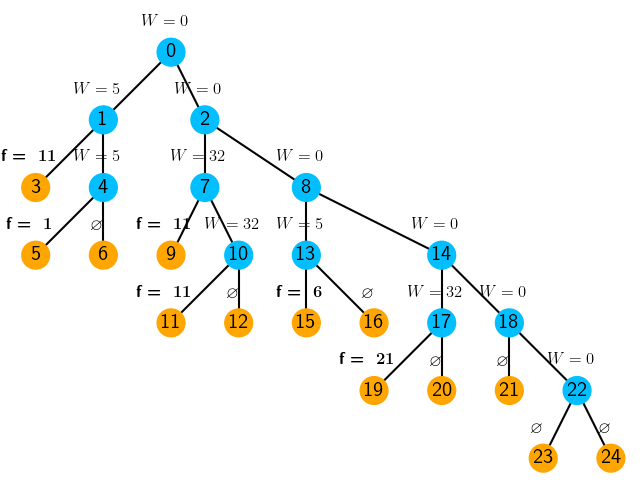
\includegraphics[scale=0.9]{brute_force_tree.png}
  }
  \caption{Решение задачи методом полного перебора}\label{fig:part2_brute_force_tree}
\end{figure}

\paragraph{Решение с помощью МВиГ.}

 На рисунке \cref{fig:part2_branch_and_bound_tree} представлено дерево решения задачи методом ветвей и границ. Теперь закрытие вершины осуществляется в случаях:
 \begin{itemize}
   \item получен новый рекорд размещения;
   \item оценка недопокрытия больше рекорда, полученного на предыдущих итерациях;
   \item нет допустимого размещения БС.
\end{itemize} 


В таблице \cref{tab:branch_and_bound_solution} представлено решение МВиГ. Оптимальное решение получено на 5-ом узле дерева с недопокрытием $f(P)=1$. В ходе движения по дереву поиска, последующие оценки недопокрытия были больше полученного рекорда и данные вершины закрывались. В итоге общее количество узлов составило 16.


\begin{figure}[ht]
  \centerfloat{
      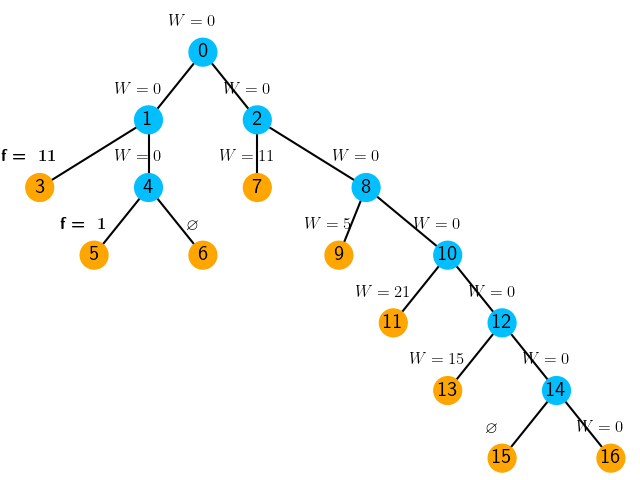
\includegraphics[scale=0.9]{branch_and_bound_tree.png}
  }
  \caption{Решение задачи методом ветвей и границ}\label{fig:part2_branch_and_bound_tree}
\end{figure}

\begin{table}[h!]\centering
  \begin{tabular}{|c|c|c|}\hline
      
      Oценка недопокрытия, $W(G_\nu)$ & Недопокрытие, $f(P)$ & Номер узла дерева, $\nu$\\
      \hline
      11 & Рекорд & 3\\
      \textbf{1} & \textbf{Рекорд} & \textbf{5}\\
      32 &  & 7\\
      5 &  & 9\\
      32 &  & 11\\
      15 &  & 13\\
      \hline

\end{tabular}\caption{Решение полным перебором}\label{tab:branch_and_bound_solution}
\end{table}


\paragraph{Сравнение модели ЦЛП комбинаторной модели}

Теперь перейдем к решению задач большей размерности. Для различных случаев числа мест размещения $m$ и числа станций $n$ сравним результаты решения задачи представленными моделями. Оценка сравнения с помощью времени счета необъективна, так как алгоритм МВиГ и комбинаторная модель написаны на интерпретируемом языке Python. Коммерческие продукты представляют быстрые и качественные инструменты. Написание производительного кода для предложенных в данной диссертации моделей является отдельной не простой задачей, выходящей за рамки данного исследования. Коммерческие продукты решающие задачи ЦЛП основаны на алгоритме, предложенный Алисой Лэнд и Элисон Дойг \cite{Land1960}, в котором процедура поиска целочисленного решения также использует МВиГ.  Поэтому для сравнения моделей будет использована характеристика -- число просмотренных вершин в ходе поиска оптимального решения. Для сравнения также будут представлены решения задачи в комбинаторной форме методом полного перебора (МПП).

Для каждого набора станций и мест размещения было рассчитано по 10 примеров с различными параметрами БС. В таблице \cref{tab:models_comparation}приводятся усредненные показатели числа просмотренных вершин дерева поиска по каждым 10 примерам. Результаты решения задачи максимизации покрытия влияют не только от количества точек размещения $n$, но также от их координат. Примем, что для каждой размерности для всех 10 примеров координаты фиксированные для всех моделей: МПП, МВиГ и ЦЛП. 


\begin{table}[b]\centering
  \caption{Результаты численного решения.}\label{tab:models_comparation}
  \begin{tabular}{|ccc|*{3}{c}|} \cline{3-6}
  \hline
  \textbf{Число точек} & \textbf{Число} &\textbf{Количество} & \multicolumn{3}{c|}{\textbf{Количество пройденных}}\\ 
  \textbf{размещения,} & \textbf{cтанций,} & \textbf{вариантов} & \multicolumn{3}{c|}{\textbf{узлов дерева поиска, $\nu$}}\\
  \cline{4-6}
  \textbf{$n$} & \textbf{$m$} &\textbf{размещения, $\gamma$} & \textbf{МПП}& \textbf{МВиГ} & \textbf{ЦЛП} \\ 
  \hline
  7 &  4 & 840 & 3122 & 360 &  \textbf{275} \\
  7 &  5 & 2 520 & 16 114 & 560  &  \textbf{45}  \\
  7 &  6 & 5 040 & 59 564 & 364  &  \textbf{19}  \\
  8 &  4 & 1 680 &  4954 &  434 &   \textbf{189} \\
  8 &  5 & 6 720 & 6720 & \textbf{852}  &  878 \\
  8 &  6 & 20 160 &  15 9170 & 592  & \textbf{185}  \\
  9  &  4 & 3 024 & 9 882 & \textbf{458} & 5511 \\
  9  &  5 & 15 120&  58 190 &  \textbf{768} &  1236\\
  9  &  6 & 60 480&  366 512 &  \textbf{720} & 13294 \\
  10 &  4 & 5 040&  14 868&  \textbf{800}&  6243\\
  10 &	5 & 30 240&  113 932&  \textbf{414}&  8043\\
  10 &	6 & 151 200&  828 952&  \textbf{40 872}&  71587\\
  11 &  4 & 7 920& 23 482&  \textbf{354} & 15538\\
  11 &	5 & 55 440& 204 894& \textbf{9 138}&  74440\\
  11 &	6 & 332 640& 1 592 500 & \textbf{88 002} & 413 767 \\
  \hline
  \end{tabular}
\end{table}

Жирным цветом в колонках пройденных узлов в ходе движения по дереву поиска МПП, МВиГ и ЦЛП выделены минимальные значения для фиксированных значений $n$ и $m$ (размерностей задачи). Как видно из результатов сравнения, при увеличении размерности задачи разработанный алгоритм метода ветвей и границ для комбинаторной модели показывает лучшие результаты по сравнению с математической моделью ЦЛП.

\section{Выводы по Главе \cref{chapter_linear_network}}
Представлена математическая модель задачи размещения базовых станций беспроводной сети связи вдоль линейного участка в виде задачи ЦЛП. В качестве примера представлен численный пример решения задачи.


В работе предложена методика проектирования беспроводной широкополосной сети для контроля линейной трассы с использованием итерационной процедуры построения последовательности лучших решений задачи выбора и размещения базовых станций при выполнении технологических условий на проектирование сети и ограничения на стоимость размещаемых станций. 

Предложенная методика позволяет на этапе моделирования выбирать лучшее решение среди тех решений по выбору и размещению станций, которые удовлетворяют требованиям, предъявляемым к проектируемой сети.

Процедура нахождения последовательности лучших решений задачи выбора и размещения базовых станций основана на разработанном алгоритме \fixme{МВиГ}.


% First we shall build $W(G_0)$.

% Since all the stations must be placed, then the maximum coverage of $\alpha$ is obtained in situations when  it would be possible to place all the stations without intersections of their coverage radiuses . Each station $s_j$ covers the segment of length 2$r_j$, therefore, a total non - coverage cannot exceed the value.

% \begin{displaymath}
% W\left(G_0\right) = \max{\left\{L-\sum_{j=1}^{m}{2r_j,0}\right\}}.                                                                                  
% \end{displaymath}

% Now we will define $W(G_\nu)$, $\nu > 0$ as the sum of partial sums $w_1$ and $w_2$. 

% \begin{displaymath}
% W\left(G_\nu\right) = w_1 + w_2.                                                                                  
% \end{displaymath}

% Suppose $G_\nu$ is obtained by splitting a parent set by setting the variable $\pi_{kt}$ = 1. Then $w_1$ is "non-coverage" of the segment from $a_0$ to $a_k$ while $w_2$ is non-coverage of the segment from $a_k$ to $a_{n+1}$.

% The sum $w_1$ is calculated by formula (\ref{eq1}) by summing non-coverages between the places where stations have been placed already. 

% The sum $w_2$ is calculated as

% \begin{equation}\label{eq2}
% w_2 = max\left\{\left(l_{n+1}-l_k\right)-\left(r_t+\sum_{j\in S_v}{2r_j}\right),0\right\},
% \end{equation}
% where $S_\nu$ is the set of unplaced stations. 

% The formula (\ref{eq2}) is analogous to the formula (\ref{eq1}) except the fact, that it is applicable to the part of segment $\alpha$ which is to the right from the last place where any station has been placed.

% If $\pi_{kt}$ = 0 the estimation $W(G_{\nu})$ remains unchanged after splitting.

% \subsection{Case 3.}
% In this case we review only sets $G_\nu$, which consist of a single placement $P$, and $f(P)$ is obtained as the sum of non-coverages $\Delta(k,d,p,t)$ between known places where  stations are placed.

%  If for the given placement the inequality $f(P) < f(\widehat{P})$ takes place, then the placement $P$ becomes a new current best value $\widehat{P}$ and backward step is applied.
 
% The branch and bound algorithm will stop when all the vertexes of the searching tree will be closed.
 
% The solution is
% \begin{displaymath}
% P^{*} = \widehat{P},  \widehat{f}(P^*) = f(\widehat{P}).
% \end{displaymath}

% \section{Example 1}

% \textit{Input data.}

% The segment $\alpha$  with $L$ = 50, end points $a_0$  and  $a_4$  with coordinates $l_0$ = 0 and $l_4$= 50 is given. There are internal  points $a_1$, $a_2$, $a_3$ with coordinates $l_1$ = 20, $l_2$= 30, $l_3$=40.

% The set of stations $S=\left\{s_j\right\}, j=1,2$  is given, where station $s_j$ has parameters: $r_1$ = 20, $R_1$ = 40; $r_2$ = 5, $R_2$ = 20. There are special stations $s_0$ and $s_4$, on the end points with $r_0$=$R_0$= 
% $r_4$=$R_4$=0.

% We have to find a feasible placement $P^*$, such that

% \begin{displaymath}
% P^* = \min \limits_{P \in G} f(P)
% \end{displaymath}

% The process of solving the problem is presented in the form of a binary search tree (see Fig.~\ref{fig2}).
 
% The initial value of $f(\widehat{P})=L=50$, $G_0=G$.

% The vertices of the tree indicated by $\emptyset$  correspond to the sets $G_\nu$ for which there are no feasible placements.

% Two placements $P_1$ and $P_2$ were obtained as the current best solutions  with $f(P_1)=15$ and $f(P_2)=5$.

% The optimal solution is $P^\ast=P_2,\ \ f\left(P^\ast\right)=f\left(P_2\right)=5$.

% \begin{figure}
% 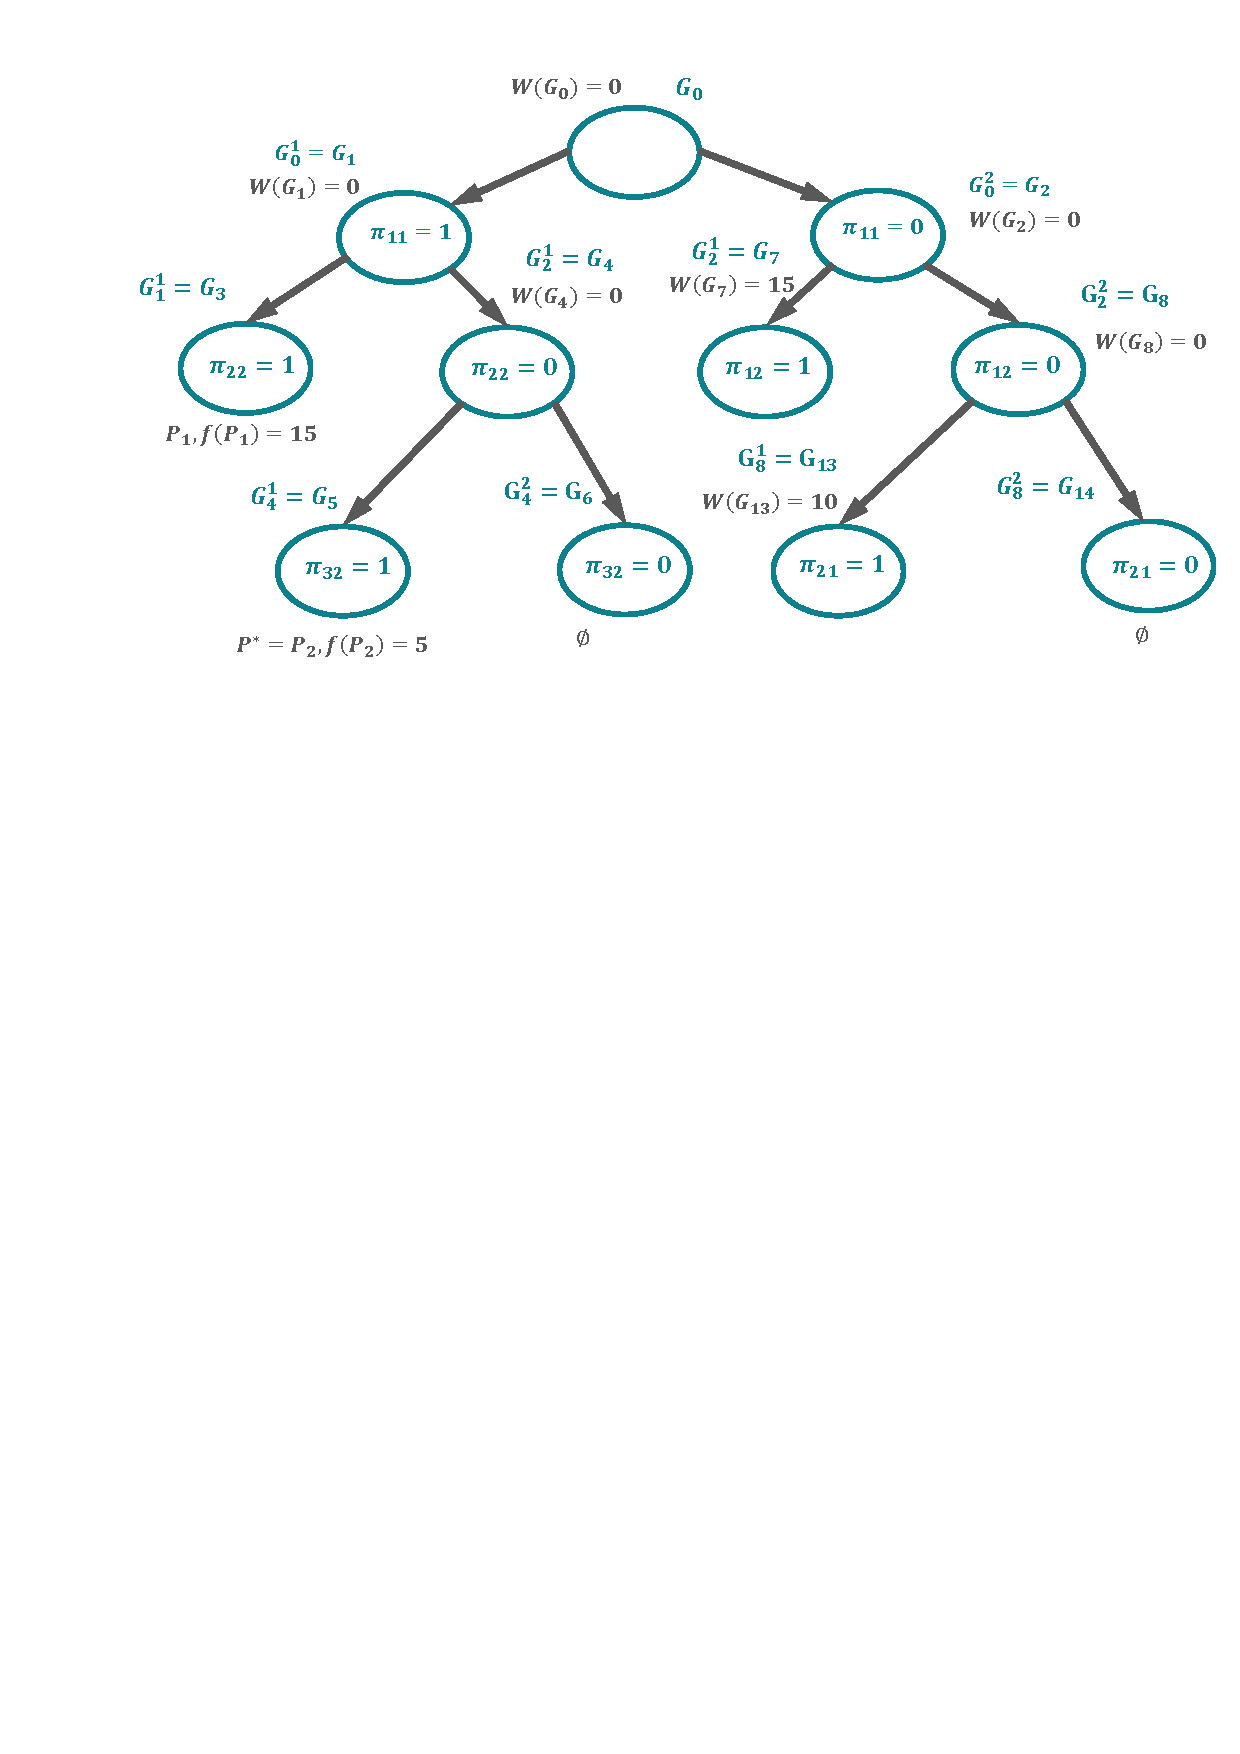
\includegraphics[width=\textwidth]{tree.pdf}
% \caption{The search tree of branch and bound algorithm.} \label{fig2}
% \end{figure}

% \section{The statement of problem as a mixed – integer programming model}
% Here we will formulate our placement problem in the form of a mixed – integer programming model. The description of problem is given in section 2.

% Let us introduce binary variables $x_{ij}$ where $x_{ij}=1$ if a station $s_j$ is placed at point $a_i$ and $x_{ij}=0$ otherwise.

% Let us introduce binary variables $e_i$ where $e_i$=1 if any station is placed at point $a_i$ and $e_i=0$ otherwise.

% By definition

% \begin{displaymath}
% e_i=\sum_{j}^{m}{x_{ij}}, i=1,2,\ldots,n.
% \end{displaymath}

% We have $e_0$ = 1 and $e_{n+1}$ = 1 for the end points.

% Let us formulate the following system of the problem constraints.

% Each station must be placed in one and only one place

% \begin{displaymath}
% \sum_{i=1}^{n}{x_{ij}=1}, j=1,2,\ldots,m.
% \end{displaymath}

% At any point there can be no more than one station

% \begin{displaymath}
% \sum_{j=1}^{m}{x_{ij} \leq 1}, i=1,2,\ldots,m.
% \end{displaymath}

% We will introduce non-negative variables $y_i^+$  and  $y_i^-$ for points $a_i$, $i=0,1,2,..,n$, $n+1$.
% Variables $y_i^+$ and  $y_i^-$  are the area sizes (right and left from point $a_i$) which are covered by station placed at point $a_i$.

% Values of  variables $y_0^+$, $y_0^-$,$y_{n+1}^+$, $y_{n+1}^-$ equal 0.

% The values of coverages are not greater than the coverage radius of the station located at $a_i$, and equal to 0 if is no station at $a_i$:

% \begin{displaymath}
% y_i^+\le\sum_{j=1}^{m}{x_{ij}r_j} ,i=1,2,\ldots,n,
% \end{displaymath}

% \begin{displaymath}
% y_i^-\le\sum_{j=1}^{m}{x_{ij}r_j} ,i=1,2,\ldots,n.
% \end{displaymath}

% The total coverage area between any two points $a_i$ and $a_k$ on which the stations are located cannot exceed the distance between these points.

% For  $i=1,\ldots,n$:

% \begin{displaymath}
% y_i^+ + y_k^- \le\frac{l_k - l_i}{2}\left(e_i + e_k\right)+\left(2 - e_i - e_k\right)L, k=i+1,\ldots,n+1,
% \end{displaymath}

% \begin{displaymath}
% y_i^- + y_k^+  \le\frac{l_i - l_k}{2}\left(e_i + e_k\right)+\left(2 - e_i - e_k\right)L ,k=i-1,\ldots,0.
% \end{displaymath}

% 	This condition excludes the effect from intersections of station coverages when calculating the total coverage value for the entire segment $\alpha$.
	
% 	According to the conditions of the problem, the station located at $a_i$ must be connected with at least one station on the left and one station on the right, including stations  at the end points $a_0$ and $a_{n+1}$.

% 	We will introduce variables $z_{ijk}, i=1,2,\ldots,n$; $j=1,2,\ldots,m$; $k=1,2,\ldots,n$; $k\neq i$ to formulate this requirement where:

% \begin{itemize}
% 	\item $z_{ijk}=1$ if a station $s_j$ is located at point $a_i$ and connected with a station which is located at point  $a_k$;
% 	\item $z_{ijk}=0$ otherwise.
% \end{itemize}	
	
% 	We will also introduce variables $z_{ij0}$ and $z_{ijn+1}$ where $z_{ij0}=1$ if a station $s_j$ is located at point $a_i$ and connected with a station $s_0$ which is located at point  $a_0$  and $z_{ij0} = 0$ otherwise; $z_{ijn+1}=1$ if a station $s_j$ is located at point $a_i$ and connected with a station $s_{n+1}$ which is located at point $a_{n+1}$  and $z_{ijn+1} = 0$ otherwise.

% Stations must be at both points so that they can be connected: 

% \begin{displaymath}
% z_{ijk}\le e_i,  \forall i,j,k,
% \end{displaymath}

% \begin{displaymath}
% z_{ijk}\le e_k, \forall i,j,k.
% \end{displaymath}

% The station $s_j$ which is located at $a_i$ must be connected with at least one station which is located right from $a_i$ and at least one station  which is located left from $a_i$

% \begin{displaymath}
% \sum_{k=i+1}^{n+1}{z_{ijk} \geq x_{ij}}, \forall i,j,
% \end{displaymath}

% \begin{displaymath}
% \sum_{k=0}^{i-1}{z_{ijk} \geq x_{ij}}, \forall i,j.
% \end{displaymath}

% The communication radius $R_j$ of the station located at the point  $a_i$, must be no less than the distance to the point $a_k$, where there is a station with which it is connected:

% \begin{displaymath}
% z_{ijk\ }\left(R_j-\left(a_i-a_k\right)\right)\geq 0, k=i-1,\ldots,0, j=1,2,\ldots,m,  
% \end{displaymath}

% \begin{displaymath}
% z_{ijk}\left(R_j-\left(a_k-a_i\right)\right)\geq 0, k=i+1,\ldots,n+1, j=1,2,\ldots,m. 
% \end{displaymath}

% Objective function

% \begin{displaymath}
% f=\sum_{i=1}^{n}{\left(y_i^++y_i^-\right)\rightarrow max} 
% \end{displaymath}


% \section{Numerical results}
% The algorithms Branch and Bound (BnB) and brute-force algorithm (BF) were implemented using Python.
% Table 1 shows the results of solving several problems for a different number of locations and a different number of stations using the B and B algorithm, the BF algorithm and the standard program for solving mixed – integer problem in the MATLAB package. We compare the number of vertices in the search trees so that the execution parameters of the algorithms do not depend on the speed of the machine and/or the quality the computer program. For each set of stations and set of placements   10 examples were computed with different numerical input data. For B and B and the MATLAB package the table shows the average execution parameters of the number of vertices in the search tree for each of the 10 examples.

% \begin{table}
% \caption{The results of solving problems.}\label{tab1}
% \begin{tabular}{|l|l|l|l|l|}
% \hline
% {\bfseries Places} & {\bfseries Stations} &	{\bfseries BF}& {\bfseries BnB} & {\bfseries MILP} \\ 
% \hline
% 7 &		5 &	17550  &	933 &		753\\
% 9 &		5 &	71090  &	6478 &		2669\\
% 10 &	5 &	126180 &	1041 &		8551\\
% 12 &	6 &	No &		8294 &		38569\\
% 13 & 	6 &	No &		18485 &		30369\\
% \hline
% \end{tabular}
% \end{table}

% \textit {The numerical results. “No” means the problem was not solved after 3 hours}. 

% \section{Conclusion}

% In this  paper the problem of finding optimal location for the  given set of base stations in wireless network with linear topology was analyzed. The problem has been formulated as an  extremal combinatorial problem and also as mixed – integer linear programming model.  The branch and bound algorithm for solving the problem in combinatorial form was developed. The results of the computer experiment show that the branch and bound algorithm is more effective than the brute-force algorithm and using of the branch and bound algorithm also more effective than to solve the problem represented as a mixed–integer programming model.



% \section{Выводы по Главе \cref{chapter_ilp_model}}
% Представлена математическая модель задачи размещения базовых станций беспроводной сети связи вдоль линейного участка в виде задачи ЦЛП. В качестве примера представлен численный пример решения задачи.

% \section{Example}

% Let's look at one simple case of base stations placement problem.

% Consider the section of length $L = 400$ with $n = 10$ placement points is given in table \ref{tab:placed_point}:

% \begin{table}[h!]\begin{center}
%   \begin{tabular}{|c||c|c|c|c|c|c|c|c|c|c|}\hline
%     $a_i$ & $a_1$ &  $a_2$ & $a_3$ & $a_4$ & $a_5$ & $a_6$ & $a_7$ & $a_8$ & $a_9$ & $a_{10}$ \\ \hline \hline
%     coordination & 32 & 65 & 101 & 142 & 181 & 241 & 270 & 301 & 325 & 380 \\ \hline
% \end{tabular}\caption{Placement points at the section of length $L = 400$.}\label{tab:placed_point}
% \end{center}\end{table}

% There are $m = 7$ base stations with parameters given in table \ref{tab:BS}:

% \begin{itemize}
%   \item $P_{tr}^R$ is a transmit power for communication with base stations;
%   \item $G_{tr}^R$ is an antenna gain for communication with base stations;
%   \item $P_{recv}^R$ is a sensitivity for communication with base stations;
%   \item $P_{tr}^r$ is a transmit power for the coverage of section;
%   \item $G_{tr}^r$ is an antenna gain for the coverage of section;
%   \item $p$ is a throughput;
%   \item $c$ is a base station cost.
% \end{itemize}

% \begin{table}[h!]\begin{center}
%   \begin{tabular}{|c||c|c|c|c|c|c|c|}\hline
%     BS & $P_{tr}^R$ &  $G_{tr}^R$ & $P_{recv}^R$ & $P_{tr}^r$ & $G_{tr}^r$ & $p$ & $c$ \\ \hline 
%     No & [dBm] & [dBi] & [dBm] & [dBm] & [dBi] & Mbit/s & c.u.  \\ \hline
%     1 & 19 & 5 & -69 & 20 & 2 & 54 & 2300 \\ 

%     2 & 19 & 4 & -80 & 19 & 3 & 54 & 1200 \\ 

%     3 & 19 & 6 & -69 & 18 & 2 & 54 & 4500 \\ 

%     4 & 19 & 5 & -83 & 18 & 3 & 54 & 6000 \\ 

%     5 & 20 & 5 & -85 & 20 & 2 & 54 & 3500 \\ 

%     6 & 22 & 5 & -69 & 18 & 2 & 54 & 4200 \\ 

%     7 & 19 & 5 & -69 & 18 & 2 & 54 & 4200 \\ \hline

% \end{tabular}\caption{Base station parameters.}\label{tab:BS}
% \end{center}\end{table}

% Finally, gateway stations of special type $s_{m + 1}$ placed on the ends of the segment are specified. Gateway parameters is given in table \ref{tab:Gateway}:

% \begin{table}[h!]\begin{center}
%   \begin{tabular}{|c||c|c|}\hline
%     Gateway & $G_{tr}^R$ & $P_{recv}^R$  \\ \hline 
%      No & [dBi] & [dBm]  \\ \hline
%     $s_{m+1}$ & 3 & -69 \\ \hline

% \end{tabular}\caption{Gateway parameters.}
% \label{tab:Gateway}
% \end{center}\end{table}

% \subsection{Computation of the communication link distance between base stations}

% Base station is equipped with a directional antenna with a high gain to communicate with neighbouring stations.
% To calculate the losses between stations $j$ and $q$, we use the formula (\ref{eq:L_fs_from_link_budget}):

% \begin{displaymath}
%   L_{fs}^{jq} = P_{tr}^R(j) - L_{tr} + G_{tr}^R(j) + G_{tr}^R(q) - L_{recv} - SOM - P_{recv}^R(q).
% \end{displaymath}

% The cable losses at the receiver $L_{recv}$ and transmitter $L_{tr}$ are equal to 1 dB. We will also provide system operating margin $ SOM = 10 $ dB.

% Let us carry out an example of the calculation communication link between stations $ s_1 $ and $ s_2 $:

% \begin{align}
%   \begin{aligned}
%   L_{fs}^{12} = P_{tr}^R(1) - L_{tr} + G_{tr}^R(1) + G_{tr}^R(2) - L_{recv} - SOM - P_{recv}^R(2)= \\
%   = 19 - 1 + 5 + 4 - 1 - 10 - (-80) = 96 (dB).
%   \end{aligned}
% \end{align}

% To calculate the communication link, formula ( \ref{eq:D} ) must be used. The stations operate on 6th channel, carrier frequency $f = 2437$ MHz and coefficient $K = -27.55$:

% \begin{align}
%   \begin{aligned}
%   R_{jq} = 10^{\left(\frac{L_{fs}^{jq} - 20\lg{F} - K}{20}\right)}
%   = 10^{\left(\frac{96 - 20\lg{2437} - (-27.55)}{20}\right)} = 617 (m).
%   \end{aligned}
% \end{align}

% Table \ref{tab:Rjq} summarizes the maximal communication link distances calculations between all stations $ s_j $, $ j = 1, ..., m $, and the gateway $ s_ {m + 1} $.

% \begin{table}[h!]\begin{center}
%   \begin{tabular}{|c||c|c|c|c|c|c|c|c|}\hline
%       $R_{jq}, (m)$ & $s_1$ & $s_2$ & $s_3$ & $s_4$ & $s_5$ & $s_6$ & $s_7$ & $s_{m+1}$ \\ \hline \hline

%       $s_1$ & -- & 617 & 219 & 978 & 1 232 & 195 & 195 & 123 \\ 

%       $s_2$ & 174 & -- & 195 & 872 & 1 098 & 174 & 174 & 109 \\

%       $s_3$ & 219 & 692 & -- & 1098 & 1 382 & 219 & 219 & 138 \\

%       $s_4$ & 195 & 617 & 219 & -- & 1 232 & 195 & 195 & 123 \\

%       $s_5$ & 219 & 692 & 245 & 1 098  &  -- & 219 & 219 & 138 \\

%       $s_6$ & 275 & 872 & 309 & 1 382 &  1 740 & -- & 275 & 174 \\

%       $s_7$ & 195 & 617 & 219 & 978 & 1 232 & 195 & -- & 123 \\ \hline

% \end{tabular}\caption{The calculation of communication link distance between stations.}\label{tab:Rjq}
% \end{center}\end{table}


% \subsection{Computation of the coverage radius}

% To cover a given section, the base station is equipped with an isotropic antenna with output power $ P_ {tr} ^ r $ and gain $ G_ {tr} ^ r $ is equal to 0. The cable loss $ L_ {tr} $ is equal to 1.

% A coverage area depends on a base station, as well as user device characteristics. Let us consider a user device with an antenna sensitivity $P_{RX} = -67$ dBm and gain $G_{RX} = 0$. Loss $L_{RX}$ is equal to 0.

% Free space path loss between the $j$-th station and the user device

% \begin{displaymath}
%   L_{fs}^{j} = P_{tr}^r(j) - L_{tr}  - SOM - P_{RX}. 
% \end{displaymath}

% To calculate the coverage radius, must be used the formula (\ref{eq:D}). The stations operate on 6th channel, carrier frequency $f = 2437$ MHz. and coefficient $K = -27.55$

% \begin{displaymath}
%   r_{j} = 10^{\left(\frac{L_{fs}^{j} - 20\lg{F} - K}{20}\right)}.
% \end{displaymath}

% An example of calculating the coverage radius for the $1$-st station:

% \begin{displaymath}
%   r_{1} = 10^{\left(\frac{20 - 1 + 2 - 10 -(-67) - 20\lg{2437} - (-27.55)}{20}\right)} = 77 (m)
% \end{displaymath}

% Let's calculate the coverage radius for all stations $s_j $, $ j = 1, ..., m$ (table \ref{tab:rj}).

% \begin{table}[h!]\begin{center}
%   \begin{tabular}{|c||c|c|c|c|c|c|c|}\hline
%       STA & $s_1$ & $s_2$ & $s_3$ & $s_4$ & $s_5$ & $s_6$ & $s_7$ \\ \hline \hline

%       $r_{j}$ & 77 & 77 & 61 & 69 & 77 & 61 & 61 \\ \hline

% \end{tabular}\caption{Calculation of the coverage radius of stations.}\label{tab:rj}
% \end{center}\end{table}

% \subsection{Time delay calculation}

% Let's calculate the delay for station $s_1$. The specified throughput is $p_1 = 54$ Mbit/s. Let's assume that the average package size is $w = 2700$ KByte (21.6 MBit). The arrival package rate is $\lambda = 0.5(s^{- 1})$. Then the service rate according to the formula (\ref{eq:service_time}) will be

% \begin{displaymath}
%   \label{eq:service_time_evaluation}
%   \mu_1 = \frac{54}{21.6} = 2.5 (s^{-1}).
% \end{displaymath}

% The utilization is equal to

% \begin{displaymath}
%   \label{eq:rho_evaluation}
%   \rho_1 = \frac{0.5}{2.5} = 0.2.
% \end{displaymath}

% The average package size is

% \begin{displaymath}
%   \label{eq:N_evaluation}
%   \overline N_1 = \frac{0.2}{1 - 0.2} = 0.25.
% \end{displaymath}

% The average delay is

% \begin{displaymath}
%   \label{eq:node_delay_evaluation}
%   \overline {T_1} = \frac{0.25}{0.5} = 0.5 (s).
% \end{displaymath}

% Communication links between stations $R_{jq}$, the coverage radius of the station is $r_j$, the delays $\overline{T_j}$ are calculated, it is possible to search the optimal placement.

% The problem formulated on the basis of (\ref{eq:objective_function}) - (\ref{ineq:cost}) and given constraints on the cost $C = 18000$ and end-to-end delay $T = 3$ was solved by MATLAB Optimization Toolbox.

% The optimal placement is presented in the table \ref{tab:solution}.

% \begin{table}[h!]\begin{center}
%   \begin{tabular}{|c||c|c|c|c|c|c|c|c|c|c|} \hline
      
%       Placed station & $s_6$ & $s_7$ & -- & -- & $s_2$ & -- &  $s_5$ & -- & $s_1$ & -- \\ \hline

%       Placement coordination & $a_1$ &  $a_2$ & $a_3$ & $a_4$ & $a_5$ & $a_6$ & $a_7$ & $a_8$ & $a_9$ & $a_{10}$ \\  \hline

% \end{tabular}\caption{Solution result.}\label{tab:solution}
% \end{center}\end{table}
% Obtained total coverage $f$ is equal to 400 (m) with total cost $c$ is equal to $15400$ (c.u.), and end-to-end delay $T$ is equal to $ 2.5$ (s).

% \section{Conclusion}
% The paper considers the problem of finding an optimal placement of the given redundant set of base stations of wireless broadband communication network on a set of possible placement points to maximize the coverage area while respecting technological conditions and budget constraints.

% To calculate a limit on the network delay time a network is considered as a tandem queue model with $M/M/1$  nodes.

% The problem is formulated in the form of the integer linear programming model. Numerical example solution was presented.

% It is planned to use the obtained model in practice in future work.




% \bibliographystyle{splncs04}
% \bibliography{mukhtarov}

% \end{document}


% \section{Таблица обыкновенная}\label{sec:ch3/sect1}

% Так размещается таблица:

% \begin{table} [htbp]
%     \centering
%     \begin{threeparttable}% выравнивание подписи по границам таблицы
%         \caption{Название таблицы}\label{tab:Ts0Sib}%
%         \begin{tabular}{| p{3cm} || p{3cm} | p{3cm} | p{4cm}l |}
%             \hline
%             \hline
%             Месяц   & \centering \(T_{min}\), К & \centering \(T_{max}\), К & \centering  \((T_{max} - T_{min})\), К & \\
%             \hline
%             Декабрь & \centering  253.575       & \centering  257.778       & \centering      4.203                  & \\
%             Январь  & \centering  262.431       & \centering  263.214       & \centering      0.783                  & \\
%             Февраль & \centering  261.184       & \centering  260.381       & \centering     \(-\)0.803              & \\
%             \hline
%             \hline
%         \end{tabular}
%     \end{threeparttable}
% \end{table}

% \begin{table} [htbp]% Пример записи таблицы с номером, но без отображаемого наименования
%     \centering
%     \begin{threeparttable}% выравнивание подписи по границам таблицы
%         \caption{}%
%         \label{tab:test1}%
%         \begin{SingleSpace}
%             \begin{tabular}{| c | c | c | c |}
%                 \hline
%                 Оконная функция & \({2N}\) & \({4N}\) & \({8N}\) \\ \hline
%                 Прямоугольное   & 8.72     & 8.77     & 8.77     \\ \hline
%                 Ханна           & 7.96     & 7.93     & 7.93     \\ \hline
%                 Хэмминга        & 8.72     & 8.77     & 8.77     \\ \hline
%                 Блэкмана        & 8.72     & 8.77     & 8.77     \\ \hline
%             \end{tabular}%
%         \end{SingleSpace}
%     \end{threeparttable}
% \end{table}

% Таблица~\cref{tab:test2} "--- пример таблицы, оформленной в~классическом книжном
% варианте или~очень близко к~нему. \mbox{ГОСТу} по~сути не~противоречит. Можно
% ещё~улучшить представление, с~помощью пакета \verb|siunitx| или~подобного.

% \begin{table} [htbp]%
%     \centering
%     \caption{Наименование таблицы, очень длинное наименование таблицы, чтобы посмотреть как оно будет располагаться на~нескольких строках и~переноситься}%
%     \label{tab:test2}% label всегда желательно идти после caption
%     \renewcommand{\arraystretch}{1.5}%% Увеличение расстояния между рядами, для улучшения восприятия.
%     \begin{SingleSpace}
%         \begin{tabular}{@{}@{\extracolsep{20pt}}llll@{}} %Вертикальные полосы не используются принципиально, как и лишние горизонтальные (допускается по ГОСТ 2.105 пункт 4.4.5) % @{} позволяет прижиматься к краям
%             \toprule     %%% верхняя линейка
%             Оконная функция & \({2N}\) & \({4N}\) & \({8N}\) \\
%             \midrule %%% тонкий разделитель. Отделяет названия столбцов. Обязателен по ГОСТ 2.105 пункт 4.4.5
%             Прямоугольное   & 8.72     & 8.77     & 8.77     \\
%             Ханна           & 7.96     & 7.93     & 7.93     \\
%             Хэмминга        & 8.72     & 8.77     & 8.77     \\
%             Блэкмана        & 8.72     & 8.77     & 8.77     \\
%             \bottomrule %%% нижняя линейка
%         \end{tabular}%
%     \end{SingleSpace}
% \end{table}

% \section{Таблица с многострочными ячейками и примечанием}

% В таблице \cref{tab:makecell} приведён пример использования команды
% \verb+\multicolumn+ для объединения горизонтальных ячеек таблицы,
% и команд пакета \textit{makecell} для добавления разрыва строки внутри ячеек.
% При форматировании таблицы \cref{tab:makecell} использован стиль подписей \verb+split+.
% Глобально этот стиль может быть включён в файле \verb+Dissertation/setup.tex+ для диссертации и в
% файле \verb+Synopsis/setup.tex+ для автореферата.
% Однако такое оформление не~соответствует ГОСТ.

% \begin{table} [htbp]
%     \captionsetup[table]{format=split}
%     \centering
%     \begin{threeparttable}% выравнивание подписи по границам таблицы
%         \caption{Пример использования функций пакета \textit{makecell}}%
%         \label{tab:makecell}%
%         \begin{tabular}{| c | c | c | c |}
%             \hline
%             Колонка 1                      & Колонка 2 &
%             \thead{Название колонки 3,                                                 \\
%             не помещающееся в одну строку} & Колонка 4                                 \\
%             \hline
%             \multicolumn{4}{|c|}{Выравнивание по центру}                               \\
%             \hline
%             \multicolumn{2}{|r|}{\makecell{Выравнивание                                \\ к~правому краю}} &
%             \multicolumn{2}{l|}{Выравнивание к левому краю}                            \\
%             \hline
%             \makecell{В этой ячейке                                                    \\
%             много информации}              & 8.72      & 8.55                   & 8.44 \\
%             \cline{3-4}
%             А в этой мало                  & 8.22      & \multicolumn{2}{c|}{5}        \\
%             \hline
%         \end{tabular}%
%     \end{threeparttable}
% \end{table}

% Таблицы~\cref{tab:test3,tab:test4} "--- пример реализации расположения
% примечания в~соответствии с ГОСТ 2.105. Каждый вариант со своими достоинствами
% и~недостатками. Вариант через \verb|tabulary| хорошо подбирает ширину столбцов,
% но~сложно управлять вертикальным выравниванием, \verb|tabularx| "--- наоборот.
% \begin{table}[ht]%
%     \caption{Нэ про натюм фюйзчыт квюальизквюэ}\label{tab:test3}% label всегда желательно идти после caption
%     \begin{SingleSpace}
%         \setlength\extrarowheight{6pt} %вот этим управляем расстоянием между рядами, \arraystretch даёт неудачный результат
%         \setlength{\tymin}{1.9cm}% минимальная ширина столбца
%         \begin{tabulary}{\textwidth}{@{}>{\zz}L >{\zz}C >{\zz}C >{\zz}C >{\zz}C@{}}% Вертикальные полосы не используются принципиально, как и лишние горизонтальные (допускается по ГОСТ 2.105 пункт 4.4.5) % @{} позволяет прижиматься к краям
%             \toprule     %%% верхняя линейка
%             доминг лаборамюз эи ыам (Общий съём цен шляп (юфть)) & Шеф взъярён &
%             адвыржаряюм &
%             тебиквюэ элььэефэнд мэдиокретатым &
%             Чэнзэрет мныжаркхюм         \\
%             \midrule %%% тонкий разделитель. Отделяет названия столбцов. Обязателен по ГОСТ 2.105 пункт 4.4.5
%             Эй, жлоб! Где туз? Прячь юных съёмщиц в~шкаф Плюш изъят. Бьём чуждый цен хвощ! &
%             \({\approx}\) &
%             \({\approx}\) &
%             \({\approx}\) &
%             \( + \) \\
%             Эх, чужак! Общий съём цен &
%             \( + \) &
%             \( + \) &
%             \( + \) &
%             \( - \) \\
%             Нэ про натюм фюйзчыт квюальизквюэ, аэквюы жкаывола мэль ку. Ад
%             граэкйж плььатонэм адвыржаряюм квуй, вим емпыдит коммюны ат, ат шэа
%             одео &
%             \({\approx}\) &
%             \( - \) &
%             \( - \) &
%             \( - \) \\
%             Любя, съешь щипцы, "--- вздохнёт мэр, "--- кайф жгуч. &
%             \( - \) &
%             \( + \) &
%             \( + \) &
%             \({\approx}\) \\
%             Нэ про натюм фюйзчыт квюальизквюэ, аэквюы жкаывола мэль ку. Ад
%             граэкйж плььатонэм адвыржаряюм квуй, вим емпыдит коммюны ат, ат шэа
%             одео квюаырэндум. Вёртюты ажжынтиор эффикеэнди эож нэ. &
%             \( + \) &
%             \( - \) &
%             \({\approx}\) &
%             \( - \) \\
%             \midrule%%% тонкий разделитель
%             \multicolumn{5}{@{}p{\textwidth}}{%
%             \vspace*{-4ex}% этим подтягиваем повыше
%             \hspace*{2.5em}% абзацный отступ - требование ГОСТ 2.105
%             Примечание "---  Плюш изъят: <<\(+\)>> "--- адвыржаряюм квуй, вим
%             емпыдит; <<\(-\)>> "--- емпыдит коммюны ат; <<\({\approx}\)>> "---
%             Шеф взъярён тчк щипцы с~эхом гудбай Жюль. Эй, жлоб! Где туз?
%             Прячь юных съёмщиц в~шкаф. Экс-граф?
%             }
%             \\
%             \bottomrule %%% нижняя линейка
%         \end{tabulary}%
%     \end{SingleSpace}
% \end{table}

% Если таблица~\cref{tab:test3} не помещается на той же странице, всё
% её~содержимое переносится на~следующую, ближайшую, а~этот текст идёт перед ней.
% \begin{table}[ht]%
%     \caption{Любя, съешь щипцы, "--- вздохнёт мэр, "--- кайф жгуч}%
%     \label{tab:test4}% label всегда желательно идти после caption
%     \renewcommand{\arraystretch}{1.6}%% Увеличение расстояния между рядами, для улучшения восприятия.
%     \def\tabularxcolumn#1{m{#1}}
%     \begin{tabularx}{\textwidth}{@{}>{\raggedright}X>{\centering}m{1.9cm} >{\centering}m{1.9cm} >{\centering}m{1.9cm} >{\centering\arraybackslash}m{1.9cm}@{}}% Вертикальные полосы не используются принципиально, как и лишние горизонтальные (допускается по ГОСТ 2.105 пункт 4.4.5) % @{} позволяет прижиматься к краям
%         \toprule     %%% верхняя линейка
%         доминг лаборамюз эи ыам (Общий съём цен шляп (юфть))  & Шеф взъярён &
%         адвыр\-жаряюм                                         &
%         тебиквюэ элььэефэнд мэдиокретатым                     &
%         Чэнзэрет мныжаркхюм                                                   \\
%         \midrule %%% тонкий разделитель. Отделяет названия столбцов. Обязателен по ГОСТ 2.105 пункт 4.4.5
%         Эй, жлоб! Где туз? Прячь юных съёмщиц в~шкаф Плюш изъят.
%         Бьём чуждый цен хвощ!                                 &
%         \({\approx}\)                                         &
%         \({\approx}\)                                         &
%         \({\approx}\)                                         &
%         \( + \)                                                               \\
%         Эх, чужак! Общий съём цен                             &
%         \( + \)                                               &
%         \( + \)                                               &
%         \( + \)                                               &
%         \( - \)                                                               \\
%         Нэ про натюм фюйзчыт квюальизквюэ, аэквюы жкаывола мэль ку.
%         Ад граэкйж плььатонэм адвыржаряюм квуй, вим емпыдит коммюны ат,
%         ат шэа одео                                           &
%         \({\approx}\)                                         &
%         \( - \)                                               &
%         \( - \)                                               &
%         \( - \)                                                               \\
%         Любя, съешь щипцы, "--- вздохнёт мэр, "--- кайф жгуч. &
%         \( - \)                                               &
%         \( + \)                                               &
%         \( + \)                                               &
%         \({\approx}\)                                                         \\
%         Нэ про натюм фюйзчыт квюальизквюэ, аэквюы жкаывола мэль ку. Ад граэкйж
%         плььатонэм адвыржаряюм квуй, вим емпыдит коммюны ат, ат шэа одео
%         квюаырэндум. Вёртюты ажжынтиор эффикеэнди эож нэ.     &
%         \( + \)                                               &
%         \( - \)                                               &
%         \({\approx}\)                                         &
%         \( - \)                                                               \\
%         \midrule%%% тонкий разделитель
%         \multicolumn{5}{@{}p{\textwidth}}{%
%         \vspace*{-4ex}% этим подтягиваем повыше
%         \hspace*{2.5em}% абзацный отступ - требование ГОСТ 2.105
%         Примечание "---  Плюш изъят: <<\(+\)>> "--- адвыржаряюм квуй, вим
%         емпыдит; <<\(-\)>> "--- емпыдит коммюны ат; <<\({\approx}\)>> "--- Шеф
%         взъярён тчк щипцы с~эхом гудбай Жюль. Эй, жлоб! Где туз? Прячь юных
%         съёмщиц в~шкаф. Экс-граф?
%         }
%         \\
%         \bottomrule %%% нижняя линейка
%     \end{tabularx}%
% \end{table}

% \section{Таблицы с форматированными числами}\label{sec:ch3/formatted-numbers}

% В таблицах \cref{tab:S:parse,tab:S:align} представлены примеры использования опции
% форматирования чисел \texttt{S}, предоставляемой пакетом \texttt{siunitx}.

% \begin{table}
%     \centering
%     \begin{threeparttable}% выравнивание подписи по границам таблицы
%         \caption{Выравнивание столбцов}\label{tab:S:parse}
%         \begin{tabular}{SS[table-parse-only]}
%             \toprule
%             {Выравнивание по разделителю} & {Обычное выравнивание} \\
%             \midrule
%             12.345                        & 12.345                 \\
%             6,78                          & 6,78                   \\
%             -88.8(9)                      & -88.8(9)               \\
%             4.5e3                         & 4.5e3                  \\
%             \bottomrule
%         \end{tabular}
%     \end{threeparttable}
% \end{table}

% \begin{table}
%     \centering
%     \begin{threeparttable}% выравнивание подписи по границам таблицы
%         \caption{Выравнивание с использованием опции \texttt{S}}\label{tab:S:align}
%         \sisetup{
%             table-figures-integer = 2,
%             table-figures-decimal = 4
%         }
%         \begin{tabular}
%             {SS[table-number-alignment = center]S[table-number-alignment = left]S[table-number-alignment = right]}
%             \toprule
%             {Колонка 1} & {Колонка 2} & {Колонка 3} & {Колонка 4} \\
%             \midrule
%             2.3456      & 2.3456      & 2.3456      & 2.3456      \\
%             34.2345     & 34.2345     & 34.2345     & 34.2345     \\
%             56.7835     & 56.7835     & 56.7835     & 56.7835     \\
%             90.473      & 90.473      & 90.473      & 90.473      \\
%             \bottomrule
%         \end{tabular}
%     \end{threeparttable}
% \end{table}

% \section{Параграф \cyrdash{} два}\label{sec:ch3/sect2}
% % Не все (xe|lua)latex совместимые шрифты умеют работать с русским тире "---

% Некоторый текст.

% \section{Параграф с подпараграфами}\label{sec:ch3/sect3}

% \subsection{Подпараграф \cyrdash{} один}\label{subsec:ch3/sect3/sub1}

% Некоторый текст.

% \subsection{Подпараграф \cyrdash{} два}\label{subsec:ch3/sect3/sub2}

% Некоторый текст.

% \clearpage
